% Comment these two lines out for HTML output
\newcommand*{\memfontfamily}{pnc}
\newcommand*{\memfontpack}{newcent}

\documentclass[openany, twoside, 12pt, extrafontsizes]{memoir}
%\usepackage{footnotebackref}
\setstocksize{8.5in}{5.5in} %Finale
\settrimmedsize{8.0in}{5.0in}{*}
\settrims{0.5in}{0.5in}
\setlrmarginsandblock{0.5in}{0.5in}{*}%%%%
\setulmarginsandblock{0.0in}{0.75in}{*}
\checkandfixthelayout

\usepackage{graphicx}

\usepackage[small]{titlesec}
\titleformat{\chapter}[display]
    {\normalfont\huge\bfseries}{\chaptertitlename\ \thechapter}{10pt}{\large}
\titlespacing*{\chapter}{0pt}{0pt}{40pt}

\newcommand{\tbreak}{
\medskip
\ldots
\medskip
}

\begin{document}

\frontmatter

\pagestyle{empty}

%-------------------------
\begin{center}
\textsc{\LARGE The Fall of King Mwefu}\\
\large The Classic Edition\\[1.5cm]
Translated from the Fo\-bwa language\\ by Allen G. Pacoitz
\null\vfill
\textsc{Whinery Press}
%-------------------------
\end{center}

\break
\null

\break
\null\vfill
\small
{
\noindent
English Translation \copyright 1909 and 1937\\by Allen G. Pacoitz.\\[0.3cm]
All rights reserved, no part of this publication may be duplicated in any form.\\[1.5cm]

\noindent
First Printing: February, 1909\\
Second Printing: August, 1934\\[0.5cm]

\noindent
\emph{The Classic Edition:} \\
First Printing: January, 1962\\
Editorial material \copyright 1962 by Robert Graft\\[2cm]
}

\noindent
Reluctantly published by\\
\emph{Whinery Press} \\
5422 Violet Drive, Antigo, W.I. 54409

\pagestyle{plain}

\chapter*{Note from the Editor-in-Chief}
Robert Graft, who is the junior editor in charge of editing this work, despises this particular translation; he has very few allies and I hope you're not foolish enough to be one of them. This translation, while differing from the original on many points, is traditional and a part of our culture in a way that the newer translations never will be (despite their accuracy).

However, Robert Graft's notes are very informative and interesting to say the least.
\begin{flushright}
\textsc{
Johnathan Concord,\\
Editor-in-Chief of \emph{Whinery Press}}
\clearpage
\end{flushright}



\chapter*{Foreword by the Editor}
\emph{The Fall of King Mwefu} is a good story; except this translation is not.
It may have seemed like a decent enough translation back in 1909 when Allen G. Pacoitz first translated it and he was the only scholar who could even read the language of Fo\-bwa.
Nevertheless, many people, who were intrigued by the story, learned to read Fo\-bwa so that they could enjoy \emph{The Fall of King Mwefu} in its original language.
And when they did, they realized that Pacoitz was inserting his own ideas and removing important content like a mad man.
The only reason this edition even exists is because despite the protest of many Fo\-bwa scholars, Pacoitz's translation is still the most popular translation in schools and in the home. 

There are now many more scholars studying the Fo\-bwa language and we now have much better translations;
do yourself a favor, drop this book right now and go out and buy \emph{The Fall of King Mwefu: Faithful Edition} from \emph{Whinery Press}, it is true to the original work, and in the oppinion of many is a much much better narrative.
Actually I don't really even care if you buy it from us at \emph{Whinery Press} or not.
As long as it's not translated by Allen G. Pacoitz you should be fine.
Note, however, that due to the nature of the Fo\-bwa language (and its total lack of word order) other publishers might call their translations \emph{King Shunwe's Descension} or any number of things. The name Mwefu itself could also be rendered (using the Pacoitz phonology) as Nweshu, Hungwe, or Fumwe; and there are also completely different phonologies out there such as the Joshua phonology where the sounds are scientifically reconstructed from phrases that are thought to be borrowed from Hebrew; so this is something to look out for in other publishers' translations. In \emph{The Fall of King Mwefu: Faithful Edition} most of the names differ from Pacoitz's because he had absolutely no consistency. Sometimes Pacoitz used the verb form of a name or worse, half the name would be in one form and the other half of it would be in another; sometimes he'd ignore putting the name in all together and substitute it with the name of a noun from English.

If for some reason you actually want to read this edition, for historical purposes or some other nonsense, then by all means read my footnotes where I point out all of Pacoitz's inaccuracies. And whenever I refer to the \emph{original} I'm referring to the original Fo\-bwa text.
\begin{flushright}
\textsc{
Robert Graft,\\
Editor for \emph{Whinery Press}}
\end{flushright}

\chapter{Maps}
\section{Pacoitz'}
I don't need to tell you that Pacoitz' map is worthless; there is only two place names written on the whole thing, the terrain is vague and there is only two rivers? I think Pacoitz just made this up, but he didn't even make it up based off of the places described in the text.
\begin{figure}
\centering
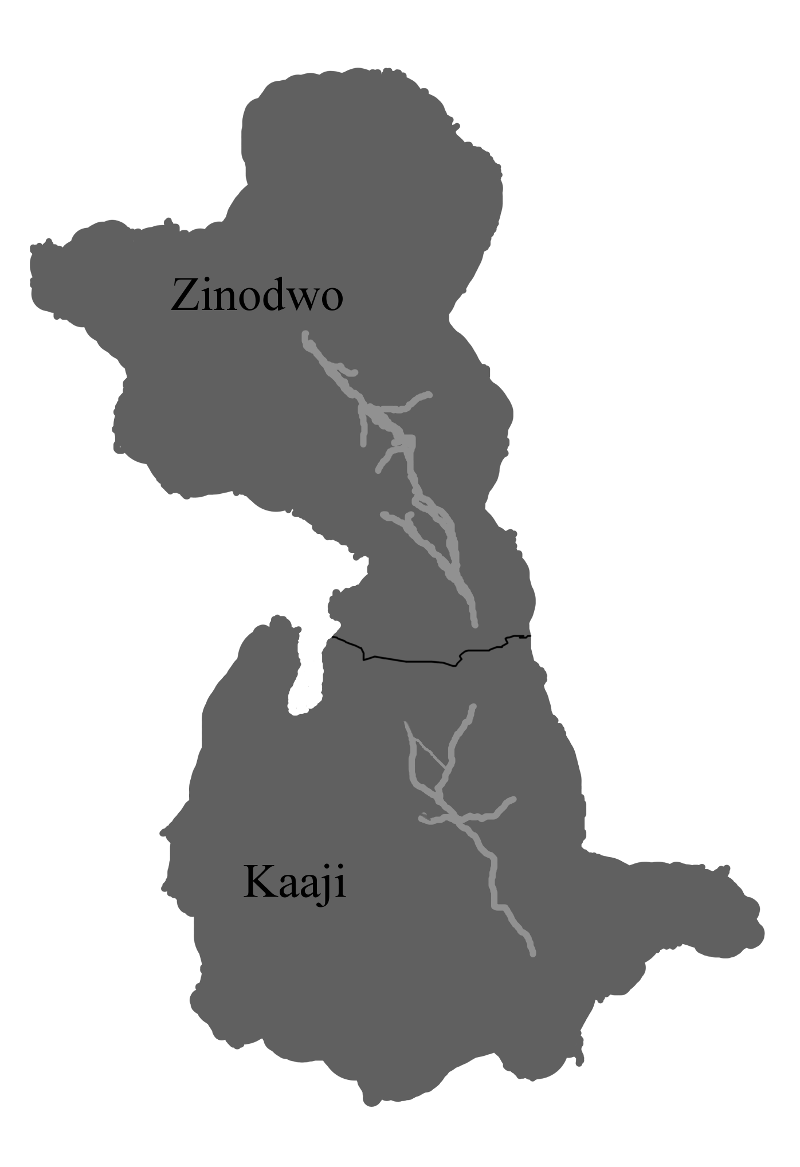
\includegraphics[width=4.5in]{Twizwa_map2.png}
\end{figure}
\clearpage

\section{Graft's}
I grew tired of looking at Pacoitz' map so I made my own using hints from the text. It's more accurate and way more informative, however, I did take some liberties.
\begin{figure}
\centering
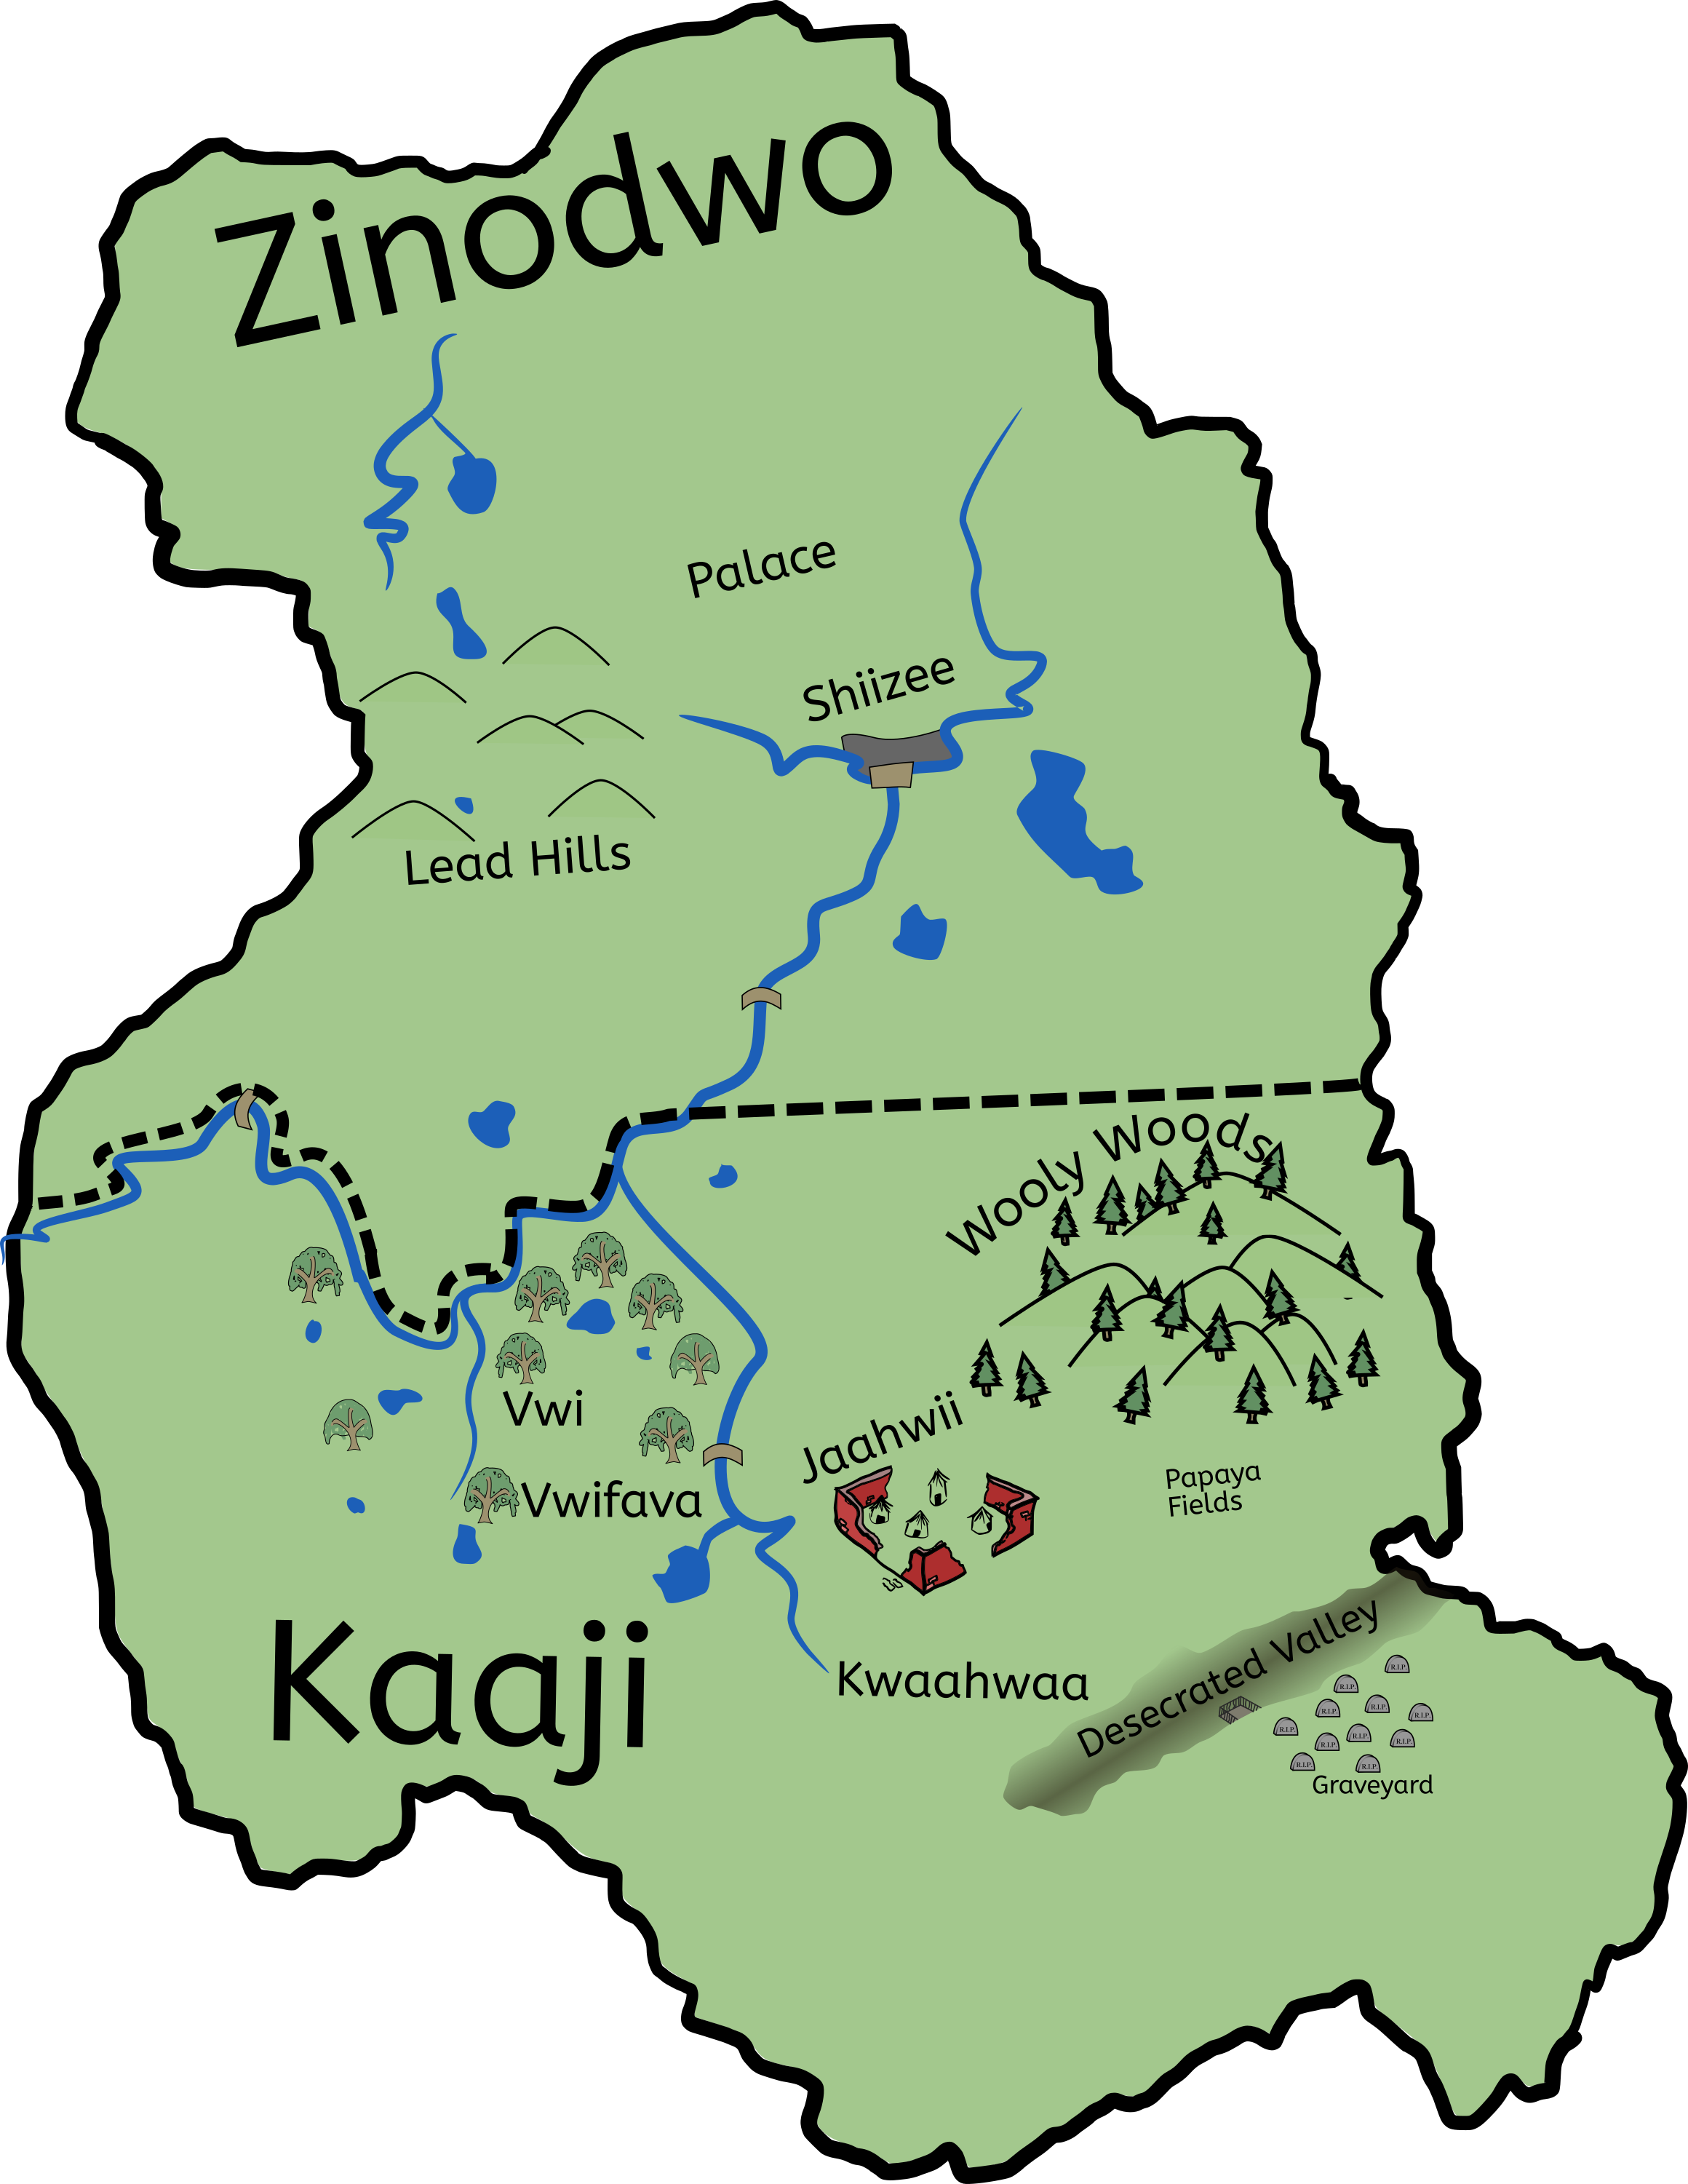
\includegraphics[width=4.0in]{map.png}
\end{figure}

\clearpage

\tableofcontents
\mainmatter
\chapter[Prologue]{Prologue
\footnote{This is Robert Graft, unfortunately, if you read the introduction you would know that I would have to pop up in the footnotes to correct things. I told you not to read this book; but since you are, the first chapter is not really a prologue by any stretch of the imagination; actually this chapter comes from the middle of the original book, but Pa\-co\-itz never was very bright and wanted to rearrange everything to make it a frame story. And the first paragraph is not even in the original text, it just comes off as Pa\-co\-itz trying to be philosophical.}
}

Others always rose up to oppose me;
I wouldn't mind so much if it was just them.
For when I count my enemies and find myself in their ranks, I realize what a wretched creature I am.
It's possible (though highly improbable) that I could overcome everyone else, but how could I possibly overcome myself since I am my own equal?

\tbreak

Finally they had done it;
the soldiers captured the armor clad rebel who had for so long defied their illegitimate and greedy rule.
The nation called Zi\-no\-dwo had been raiding the poor country (The country wasn't so poor until after it got raided) of Kaa\-ji for almost a decade.
Many heroes had risen up to stop the soldiers of Zi\-no\-dwo, but this one was the best -- this one also just happened to be me.

They led me up the scaffold, I could hardly walk since they had me bound with so many nets and chains. I knew what was going to happen, they began to tie the noose; I was to be killed like all the heroes before me. But then a soldier removed my helmet.

``My Lord!? He's our King!'' Shouted the soldier in bewilderment.
For I was.
And now it was clear that the very same person that was giving the orders was also the one thwarting them.
But that didn't make any sense, what would I the king have to gain by losing the war? Surely not money because however much Kaa\-ji was paying me I could get more by simply taking it from them.

\indent ``Explain yourself.'' Said the king's second in command.
(Pardon my confusing habit of switching point-of-views, as a king this tends to happen: like using \emph{we} in place of \emph{I})
\footnote{Note that in Fo\-bwa, kings do not talk about themselves by using \emph{we} or anything similar, but Pa\-co\-itz doesn't care about historical accuracy as long as he can get a laugh.}
I was very much ashamed of what I had done.
The crowd consisted mostly of Kaa\-jin
\footnote{This means people from the country Kaa\-ji which scholars tell me is Fo\-bwa for ``weak (soft) place''.} with some of my Zi\-no\-dwan
\footnote{People from Zi\-no\-dwo, Fo\-bwa for ``rare place''.} soldiers to control them. Despite this, all the people -- in unison -- began to chant, ``Explain!'' and kept on screaming until, ``If you'll be quiet I might just let myself explain!'' I shouted. 

I knew that both sides wanted to kill me; so I began to tell my story.

\chapter{Bamboo Poles}

As you know, I am Mwefu the king of Zinodwo. My reign began 12 years ago when I was 27 years old. I am now 39 years old and for the past six years (under my rule) my country had destroyed and robbed this country of Kaaji, killing whoever stood in our way.
We knew our conquest was wrong, but we loved the spoils thereof too much.

One day, in the 3rd year of our conquest,
\footnote{In the original the exact date is there, but Pacoitz never bothered to learn to read the Zinodwo calendar.}
a group of 20 of my soldiers robbed a fruit merchant. They brought the merchant before me in my tent.

``Tell me,'' said the boy, who was also the merchant, ``is it right to rob a citizen of Zinodwo? If it is, then why not do it in your own country?''

``You are from Zinodwo?'' we asked.

``Yes.''

``What are you doing here and why haven't you returned?''

The boy muttered something; he wasn't nearly as articulate when he didn't know what he wanted to say. \footnote{The original goes on to talk about how he had planned what he was going to say on the way over, and like with all times when you plan what you're going to say, the other person says something unexpected.}

``Well?'' I interrupted.

``I was adrift in the flood five years\footnote{five years and ten months actually.} ago and I tried to get back. But your guards wouldn't let me back into Zinodwo because I didn't have my papers.'' responded the boy.

``So you'd like it if I had my soldiers escort you across the border?''

The merchant looked at the ground and fidgeted nervously.

``Well, I have a livelihood here, and I don't know if my family survived the flood. No offense, but I like this country very much and would like to know I have friends to go back to in Zinodwo before I leave.'' said the boy.\footnote{He was hardly a boy since according to the original, he was 15.}

``If you give me a list I'll have some of my soldiers check for your friends and relatives. What is your name?''

``Paavo.'' said the merchant as he started writing down his friends and family's names.

``Paavo, with a name like that you must be pretty timid.\footnote{\emph{Paavo} is Fo\-bwa for ``weak heart'' which figuratively means \emph{lazy}, not \emph{timid} as Pacoitz's bad translation skills might imply.}''

``I suppose. May I have my money and fruit back now?''

``Well, perhaps, but it has been 3 months\footnote{Pacoitz actually had this number translated properly, I suppose even he gets lucky.} since I've spoken to a Zinodwo who wasn't my soldier. I'd like to see you again. So I'll give you back your stuff and more if you come back tomorrow.''

``Thanks. But I just want what was taken, I don't need \emph{more}.''

I felt guilty for stealing Paavo's stuff, never had I felt so bad about what before I had merely considered acquisition of wealth. But now I had robbed one of my own people. So I gave Paavo back his possessions and sent him home. It wasn't just I who benefited when we raided Kaaji though, it was my whole country, for every bit of treasure I brought back, I only kept 1\% of it of myself, the rest got evenly distributed across the country; this made me very popular, and also made me wonder if I'd still be if I ever stopped plundering Kaaji.

Before the day had passed, my men and I had robbed three more merchants and 21 odd homes (They were odd because their number was not divisible by two\footnote{Oh no. Here's another terrible pun that Pacoitz added.}).
It was the first of the month, so we loaded up our horse drawn carts with all of this month's spoils and headed towards the river where we'd meet one of my ships. From there we would load up the ship and the ship would take the loot and distribute it across Zinodwo, making all my people richer.
But as we were traveling the path that went through the northern woods, the figure of a man appeared. He was clad head to toe in corroded copper; the blue-green armor was not in the least bit threatening; that is till after he ran towards us.

My guards shot arrows at him, but it was of no avail, the arrows glanced off without slowing him down. In and out of the trees he ran, very quickly for someone in what must have been a very very heavy\footnote{The original says 110lbs.} suit. When he reached the carts, he pulled the pins off the axles on one side of each of the carts. This of course caused the wheels to fall off, tipping the carts over and spreading the jewels and coins all over the mossy ground. My soldiers tried to kill him with swords, but the copper armor was stronger than steel and the blades could not cut or dent it. 

Not wielding a sword of his own, the copper man caught a swinging blade in his armored hands. He twisted the sword out of the soldier's hand and struck him with the hilt before throwing the sword into a nearby pond where it sank to the bottom. He proceeded to do likewise with six others. So, seeing swords were of no use, three of my soldiers tackled the copper clad soldier. He could not win in a simple wrestling match, so he squirmed out from under their grasp and ran back into the deeper part of the woods.

``That,'' said Twizwa,\footnote{Fo\-bwa for ``heavy servant''. Names in Fo\-bwa are given to you when you're born, (though sometimes they are changed, as it was with Mwefu) so it's most likely that Twizwa was a fat baby.} my head soldier, trembling, ``was a man we killed last year. He ran our ship aground, so we tied him up and burned him at the stake while he was yet in his armor. Then we removed his ashes and cast the suit into the river.''

My heart sank at these words that Twizwa said, but I didn't want to admit this.

``So what if he's a ghost? If we killed him once, we can kill him again.'' said I.

We had lost a great deal of time, and the journey would not be able to be completed till the next day, so my men stopped for the night.
We picked up the treasure and left it in the carts (which we kept the wheels off of to prevent the pins from being pulled out and toppling the cart) and I left 30 men to guard it for the night.

I, surrounded by the rest of my guards, went back along the path to our camp and I retired to my tent and slept, but not too well.

\tbreak

When the sun rose, I got up and remembered Paavo and the note he had written me. I gave word to one of my messengers to go aboard my treasure ship before it left that day to Zinodwo and go inquire about the list provided by Paavo. 

Well it was time for breakfast, so I ate like a king. I had eggs, rhubarb crisp, roasted almonds, and toast with apricot preserves. \footnote{Yes the ``ate like a king'' is not in the original, Pacoitz is pitifully trying to be funny again. And not even the most learned Fo\-bwa scholars can figure out what the king ate for breakfast; but they are fairly certain that he didn't have any of the things that Pacoitz claimed he did.}
I was glad that I wasn't like the poor people of Kaaji who could only afford disgusting food such as escargot and grass-fed beef. \footnote{Pacoitz is going for irony here, but none of this is in the original! Pacoitz does not belong translating great works if he is going to behave as if he were the writer!}

I waited for Paavo to show up; and waited.
It was half past noon when I finally considered that perhaps he was not coming.
Why should I have regretted taking his possessions if he was just a lazy
\footnote{See \emph{footnote 5}.} greedy merchant with no respect for the crown?!
Truly if anyone deserved my wrath it was --- and my doorman appeared.

``Paavo is here to see you,'' he said, ``shall I let him in?'' My anger subsided.

``Why yes. Take him that painting of me.\footnote{Another superfluous joke.} Just kidding, let him in.'' Paavo entered, eating an apricot\footnote{According to his biography, Pacoitz was very fond of apricots and tried to find ways to put them in everything he did.}.

``Would you like some?'' he said, wiping the juice off his chin.

``No thank you. It is good for you to be in my presence.'' We said.

``What do you mean by that?'' asked Paavo.

``Oh, it's just kingly speech. It means `I'm glad to see you.' ''

``Why do it at all?''

``Because we are the king ---''

``You and \emph{I} are the king?''\footnote{Pacoitz and his English-based foolishness again.}

``No, I alone am king, and the king only uses superior (often confusing) speech because he is always right.'' Well, at least I wanted to believe that I was always right.

``What about people that disagree with you, you the king?'' said Paavo.

``They die of course.''

``Sounds harsh.''

``It's necessary so that the king can remain in power. By the way, I sent my messenger with the list of names you gave me.''

``Thanks, I appreciate it.''

``Have you ever fought before, Paavo?''

``No, not really.''

I picked up two bamboo poles and tossed one to Paavo. I told him to fight me, but he could not wield the rod very well. I knocked it out of his hands many many times. Whenever I went to strike him, he caught my pole with his hands instead of deflecting it with his pole.

``Hold on,'' I said, ``if these were real swords instead of bamboo poles you would not be able to do that, your hands would be chopped off. You can't just catch swords in your hands.''

``I know,'' replied Paavo, ``it's just the first thing I think of when something is flying at me.''

We tried again, and again; we fought all day into the night. He was getting better, but he was still bad. At least now he wasn't catching the bamboo in his bare hands. I won every single time (That doesn't really reflect much on his inability though since I'm very good with swords).

``Are you coming back tomorrow?'' I
\footnote{I knew one high school English teacher who read this version of the book, and she saw king Mwefu's lack of using the royal ``we'' around Paavo as proof that Mwefu feels more like a normal person (and less like a king) around Paavo.
But there's absolutely no evidence in the original that the King feels more normal around Paavo at this point. 
Even Pacoitz himself admitted that he only translated it that way because it was too confusing when the king used ``we'' in situations where it could be confused to be something other than the royal ``we''. To mistake Pacoitz for a great translator is to deny the truth of his destruction of real literature.
} asked.

``I don't know.'' said Paavo, ``I'll probably be too bruised and sore in the morning to even get up out of bed.''

So Paavo went home (wherever that is). My soldiers arrived back with their spoils. I went to bed.



\chapter{Music}

Nothing of importance happened the next day. Paavo did not come to visit me; likely because he was sore from fighting me all night.

The day after that, however, Paavo arrived for breakfast. He didn't care much for the wine or finer foods, instead he ate apricots. We then practiced fighting again with bamboo poles. I won as always, but he was showing promise.

``Your highness,'' said Twizwa as he entered my tent, ``the time for the raid draws near as a fish eats the bait.'' Twizwa was a far better poet than anyone in my kingdom.

Some question my choice in putting Twizwa in command of our army since he's really not a very good fighter. When we first became king,
\footnote{Pacoitz omitted the part of the story where his former head soldier, Bwaa tried to kill king Mwefu and was thus put to death. In fact in the original there was a whole chapter about it, and besides developing Twizwa's character, it made Mwefu's choice to elevate Twizwa much more credible.}
I asked Twizwa when he was just my page, we asked him, ``Twizwa, you are wise beyond your years, tell me, who would you put in charge of my military?'' and he replied with, ``If I were the king, I would search my kingdom for the one whose grasp of language were unparalleled, whose way with words was unmatched.''

The truth is that words are more useful for controlling than might is, and I already am the greatest fighter we've ever faced, so why would I need another great fighter if he's just going to command rather than fight anyway? I don't even see why I was made king, just because I won a tournament? Because I took down the ten best warriors in the country? That's just how the system for the election of kings in Zinodwo works. But we're glad that's how it works because the conveniences and power of being king are most delightful.
So if my second in command should be good with words, then who else can speak as Twizwa can?\footnote{See Appendix \ref{rotshift}} So I put him in charge of the military.

I sent Paavo home and we went on the raid with Twizwa. We were camped in, and still were taking resources from the village of Vwi in Kaaji. We marched through the trees to the west and came to a place where four brick houses were.

We divided into five groups; four to rummage each of the houses, and one to play some triumphant trumpet music. One of the most important parts about being king is having a presence that demands respect.
The people were forced out of their homes and the beautiful music made the feat seem glorious. They were about to all be killed, but then I noticed that someone else had joined the band, a flute was echoing the theme that our musicians were playing. It got closer and closer, till the blue-green copper clad figure appeared atop the bluff; he was playing a rather large bamboo flute.

My trumpeters stopped, and I told my soldiers to apprehend the flute player. They shot arrows at him, which of course bounced off his armor. He did not stop playing that flute. He made his way down the cliff, hopping from rock to rock. Then using an arrowhead in his free hand, he cut the ropes that held the horses to the cart and scared them off.

``He's taunting us, isn't he? He's like a shrew wrestling a snake.'' Said Twizwa.

``Just get the nets and remind the soldiers that even though his armor makes it impossible to cut him, blunt blows should still hurt.'' I said to Twizwa.

``You're assuming he's made of flesh and blood and all the other necessary organs, and not a ghost.''

Twizwa gave the commands that I told him. The soldiers beat upon the rebel with their swords, ruining their edges in the process; nevertheless it seemed that it was having effect, because he was knocked to the ground. They were about to tackle him when he got up and snatched one of the swinging swords. Lo, and behold, he could wield a sword now. He disarmed and wounded many of them (They weren't wearing full armor as he was because it would be too heavy to be practical). Meanwhile, the people who we had planned on killing had fled into the woods and no soldier was left to stop them because they were too busy either fighting the rebel or playing music.

Then he too disappeared into the woods. Not one of my soldiers could catch him.\footnote{Pacoitz fails to mention that the soldiers rode horses. But with all the trees and cliffs, and paths which are too narrow for horses to go through, the soldiers were at a disadvantage; and he was far too fast to be apprehended on foot.} If I hadn't believed he was a ghost before, I believed it now, and it filled us all with fear.

A resistance then broke out and the people whose homes we had forced them out of had come back with a militia and they drove us out of there before we could claim any of their gold or silver. I really hated that rebel.

Then the most terrifying thought occurred to me; neither the rebel nor Paavo could wield a sword when I first met them, but after I taught Paavo how to fight, the rebel showed fighting skill too. They also caught weapons in their hands. Was this enough grounds to prove they were the same person, that my good friend had betrayed his own country and was fighting for the enemy? No, no, it couldn't be, Paavo was far too frail to be such a warrior.

\tbreak

I awoke the next morning to Twizwa giving a speech about the proper way to kill an enemy or something like that.\footnote{In the original, Twizwa's speech is actually about ghosts and about how it might be possible to defeat the copper clad warrior by utilizing various supserstitions. It was an amusing and interesting speech, and it is inexcusable for Pacoitz not to put it in. To omit this part leaves out a lot of the original comedy (which was actually funny, unlike Pacoitz's puns).}
Forgetting my suspicion that Paavo might be a traitor, I taught Paavo how to wrestle; he learned very quickly and over the course of that week he got very good at it. My soldiers made some raids throughout that week without me, but each time they came back with less and less gold and more stories of the ghost of the copper clad rebel. I was sick of it, but I was too afraid to die in battle against an invincible adversary. But suppose it was Paavo? I needed to go on one last raid to find out.

So we went north towards the river and stole some silver from the people there. But the copper clad rebel ran up like usuall and my soldiers tackled him. For a moment he was on the bottom of a pile of four soldiers, but then I saw him, flip over soldier after soldier till he was at the top of it, twisting arms in a way that prevented any of them from moving. All the soldiers quaked in fear.

So now I knew that this rebel was indeed Paavo, using the same techniques I had taught him. I knew he was not a ghost, so I drew my sword. We fought, just me and him, but I was a great swordsman and I disarmed him. Then I sliced the hinges off the breastplate of his armor, leaving his chest exposed with only his yellow shirt to protect him. Then, I stabbed him through the left side of his chest. Piercing where I knew his heart to be. The music my soldiers played was triumphant, but my heart\footnote{I hate this word, it's so vague. It's definition varies to the point that it means nothing. It's clich\'{e} and Pacoitz is a fool for using it. A better word for this context would be ``emotions''.} did not listen and instead played a dirge. 

The rebel collapsed and his once quick body became as slow as the dirt. We let him lie there. I knew it was Paavo, I had no need to remove his helmet. I almost regretted killing him since he had been good company.
I figured that if anyone found out that the rebel was Paavo I'd look like a fool for befriending the enemy;
So we commanded that no one touch the body, under punishment of death. Then I realized that with the body sitting there, anybody (whether they were my soldiers or not) could take off the armor and see who was in it when I was not looking; it'd be best if I brought the dead rebel back to my camp where I could come up with an excuse to remove the body from the armor myself and keep his identity a secret.

``Let's take the body with us.'' We said.

``But you said not to touch it.'' An obnoxious soldier replied.

``Oh, yes, you're right.'' I didn't want them to think I had changed my mind about that, so I picked up the armored rebel; he was heavy, but the exertion was worth not going back on my own orders.

We then finished the raid and went back to camp where we celebrated our victory; not even the death of a good friend can stop me from enjoying good wine and admiring good gold. After that though, I had a casket made and set in one of our supply tents. Then I placed the copper rebel inside it and locked it with a padlock. But I forgot to tell someone to bury it.

\chapter{Epiphany}

Several days passed and we were nearly finished plundering the city of Vwishaja\footnote{``Yellow child.'' However, this word is rendered improperly because the different syllables are in different cases for apparently no reason; it should be \emph{Vwifava} or \emph{Jwihaja} if we conjugate it into a verb like \emph{Kaaji} is.}. But as I was doing some shopping\footnote{More like stealing.}, I saw Paavo, selling fruit as he always did.

``Hey, sorry I haven't visited in awhile. I've been kinda busy selling fruit. Business has been booming.'' He said. I did not know what to make of this, I was absolutely certain that Paavo was the copper rebel, but I'd killed him, stabbed him through the heart, how could he still be alive?
Perhaps he and the rebel were two separate people after all.
Could it be that I'd misjudged him and he'd been my ally all along?
Or maybe he really is a ghost and that's how he survived -- No, no! Paavo is no ghost.

``What kind of fruit would you recommend?'' Said I to him.

``Well, there's apricots.'' He replied.

``No, I mean good fruit.''

``You don't like apricots?''

``No, not really. I'll take six bushels of oranges.'' I said as I handed him six small nuggets of gold.

My men and I went on our way, and ate all the oranges we had bought in a matter of minutes. Then we went back to camp. The first thing I did was hurriedly go to the supply tent to double-check that the rebel was still inside it. But he wasn't, and the casket looked as if it had been kicked apart from the inside out. The padlock was still on it, but since there was a gaping hole in the top of the coffin, the lock had done no good. Now I know someone did not steal the body, the splinters from the hole were pointing outward, so the rebel must have come back to life. But even if the rebel had come back to life, that didn't mean it was necessarily Paavo.

I didn't know what to do, so I showed Twizwa the broken casket.

``That rebel will not stay dead.'' Said Twizwa, ``But that matters little now I suppose. From what I know, ghosts are usually local, they only haunt near the location from whence they were slain. If we were to go to the next town we might find all our ghosts problems to be gone. And besides that, we're finished with this town anyway.''

\tbreak

The next day our ship was blowing its horn in the harbor. Apparently they were ready for another shipment of spoils. I gathered most of the men and we brought our horse drawn (apparently horses are very good artists\footnote{Another clich\'{e} pun.}) carts out to meet it. My soldiers were on the look out for the copper warrior. They were very frightened at the thought of ghosts, and I was too; I was a much better fighter, and it's very unlikely that'd I lose a fight to it, but with all the coming back from the dead, sooner or later he might get lucky and I might get a headache, and I might lose. I hoped what Twizwa said about ghosts being local was true and not merely wishful thinking. It'd be dreadful to move to the next town and have to kill it all over again, and again, and again.

As the saying goes, speak of the devil and he appears.\footnote{In the text, both Pacoitz's and the original, no one was talking about ghosts (though they all were thinking about them). And this line, besides being bad even before it became overused in everything, is not even in the original.} One of the carts tipped over and lo, the copper clad rebel had been in the cart, hiding under the money the whole time and had pulled the pins off of one side of both axles. He then leaped into the next cart and proceeded to tip it over as well.

The rebel's breastplate was still broken off and he worked hard catching swords and blocking arrows to prevent them from hitting his chest. Then when my men remembered to wrestle him, he knocked several of them down the hill that the path was going down. Then, running fairly fast, he disappeared into the woods. He only managed to tip over two of the carts, so the other one was still standing.

Then we had to fix the carts. While we were fixing them, that messenger that I had sent earlier arrived.

``I found out what you wanted me to look into about Paavo.'' The messenger said. And he went on to explain that Paavo's family was all missing as far as he could find out, but he did find some old friends of the family; they told him that when Paavo was born his parents could barely feel his heart beat, so they named him Paavo which means ``weak heart.'' No sooner had they named him though, when they realized that his heart, as it turns out, was on the other side of his chest. Paavo did not have a weak heart after all, they just checked for a heartbeat in the wrong place. But this didn't matter, because by the time his parents realized this the name had stuck.

This all made sense then. The teal colored copper clad rebel\footnote{Pacoitz constantly renders the same Fo\-bwa phrase regarding the rebel as something different each time. His unsurety is nauseating.} was Paavo, and because he was Paavo he learned as Paavo learned, and when stabbed in the left of the chest he did not die, because his heart was on the opposite side. The warrior was no ghost, and neither was Paavo.

But what was I to do? Was I to betray Paavo as he betrayed me?
No, I liked him.
I couldn't bear to bring upon him that much disgrace and to lose him to death a second time.
As long as no one found out, I would be saved from the shame (and possible revolt against me) from befriending this rebel. I would then tell no one; not even him, because then no one would ever hear me say anything to implicate myself in such a crime against Zinodwo. I was still going to make sure that Zinodwo got plenty of spoils, but I also wanted Paavo to feel like he was doing at least something noble to stop our conquest.

\tbreak

Because Twizwa kept nagging me about ghosts and how foolish I was being for staying in this village, we left Vwishaja and headed toward Jaa\-hwii\footnote{Fo\-bwa for ``tall and solid.''}. The city had thick walls and it had a lot of archers. But we assembled trebuchets and launched many boulders at it. We sieged it for a few hours; it didn't take long.\footnote{In the original, the city had been in ruins since the King had besieged it the year before and he had only now got around to plundering it. It is very foolish of Pacoitz to think that anyone could siege a city in just a few hours.} The wall was now in shambles and many of the buildings too. With the archers all defeated we marched into Jaa\-hwii.

On the way, a beggar stopped us, he laid right in the road. He was old and he was scruffy and he asked us for some alms.

``No,'' We said to the old man, ``we don't support beggars, it's not a good way of living.''

``You are the king of Zinodwo, aren't ya?'' Replied the beggar. Then he burst out laughing uncontrollably. It took a good minute to stop him.

``Why are you laughing?'' Asked Twizwa while he violently shook the man.

``The king of the other country said he don't support beggars. Well, that's funny indeed because he created two whole countries of them. You robbed my country of Kaaji blind and made us into beggars, and then you know the rest.''

``Know the rest of what?'' I asked, ``I do everything to stop begging in my country. I even went as far as to give 99\% of all I get on my conquest here to every constituent of Zinodwo.''

``And that's why they're beggars.\footnote{Pacoitz is bad at formatting dialog, to clarify, this paragraph is said by the beggar.} Because they don't have to work for the money they get, a great lot of them take all the money they get and spend it on casinos, women, and strong drink. And then they have no money left for food so they resort to begging in the streets. So I say unto you that you must like beggars, you've created an awful lot of them, and you like supporting them too. So give me some gold.''

``That's completely ridiculous! All of that is unfounded.'' Said Twizwa.

``I'm not moving off the road till you give me something.'' Said the beggar.

Not being able to put up with it, we gave the beggar a nugget of gold, however, he still did not move.

``Hah! I knew you were a beggar lover.'' He said.

``Come on, we gave you some gold, now move!'' I yelled at the beggar.

``Can't move, I'm a cripple.''

I dragged the beggar off the road and tossed him into a thorn bush. He did not know how to act before a king, and he had offended me by accusing me of making both Zinodwo and Kaaji countries full of beggars. I knew he was wrong -- I really hoped he was.

We went into the city and pitched our tents, and slept.



\chapter {Marred and Pierced}

``King, the beggars have showed up in great numbers. They're stirring up a riot.'' Said Twizwa, waking me up.\footnote{There's a gap in the narrative here, four days have actually passed since they set camp in the city.}

``Drat,'' We said, ``you give a beggar some money, and now the whole world knows where to go for hand-outs. Tell them we're not giving them anything!''

``I did that already. But they are insisting.''

``Drive them away!''

``Sir, there's at least 3,000 of them.''

 ``3,000, that is a mess. Well, we have 416 men, they could probably take out no more than six men each -- We're dreadfully outnumbered. Go fetch that beggar from yesterday. I'll bet he's in this somehow.''

They brought the man before us.

``Why is that crowd here?'' We asked him.

``Alms, what else?'' He replied.

``There must be 3,000 people out there.'' I said, ``You sent them didn't you? Don't bother lying, I know you did. What's it going to take to make them leave? And please don't say `alms.'" We said.

``You're cursed.'' Said the beggar, ``Last night\footnote{``Two nights ago'' in the original.} I beheld a man wearing wooden armor, marred and full of arrows. He went from town to town telling all the beggars to come here and recieve treasure from you, the enemy king.''

``That's ridiculous.'' Said Twizwa, ``How can a cripple see what happens towns away when he cannot walk? You're a liar in everything you say.''

``Well, that may be true.'' Said the man, ``But I only stretch the truth when it falls short of reality, in order that it might be more so.''

``More what?'' We asked.

``More itself, more truthfull.'' Replied the beggar.

``That doesn't make any sense.'' Said Twizwa, ``The truth doesn't ever fall short of reality, because reality is truth. And when you stretch the truth you are making it into a lie.'

``But when I stretch it, there's more of it and thus more truth.\footnote{This whole banter about truth only applies to English, and so you can guess that it is another pathetic addition by Pacoitz.}'' Said the man.

``We're done talking with you.'' We said.

``In the last town you were in, a rebel, clad in copper, opposed you and made your raids difficult--''

``Who told you of this?'' I interrupted.

``Twizwa told me.'' The man said.

``I did no such thing.'' Twizwa said.

The beggar began to laugh obnoxiously, ``Since Twizwa first opened his mouth, I saw that he was a master of words, that can hide messages in speech. Apparently, by pure accident, he puts secret messages into everything he utters.\footnote{Pacoitz omits the beggar's backstory about how the beggar was lazy and spent a lot of his time playing with words and could hear the rotations of a person's speech.} He's so good he doesn't even realize what secrets he's telling (which most people won't catch) in his everyday conversation.''

Twizwa blushed and said, ``King! He could have heard about that copper rebel from \emph{any} of those beggars.''

This beggar was a liar. But was there any truth in anything he said?

``The spirits of those rebels you killed are rising from the grave to stop you; their blood cries out from the ground.'' Said the beggar, ``First the copper, now the wooden. If you leave to another town, another warrior slain in battle will meet you there. You couldn't kill the first; this one too shall haunt your every step. You want to know why those beggars are there, because the ghost of this rebel invited them.''
 
``I don't care why they're here.'' We said, ``Can you get rid of them?''

\tbreak

``Pardon me,'' Said Twizwa, interrupting my story, ``but isn't it foolish to think that chest wounds are only fatal when they hit the heart?''

``Twizwa, why didn't you bring that up when I was telling that part?'' I responded, shifting the chains to make myself more comfortable.

``My mind wanders, I only thought of it now.''

I was still on the platform telling my story,\footnote{Here Pacoitz returns back to the frame story he contrived. If this is hard to understand it's because Pacoitz's ability to weave a narrative is very weak. If you remember back in the first chapter, the king is telling this story and this question from Twizwa is a disruption to his telling of it. It makes no sense to have this interruption to Mwefu's story be here instead of when the event actually happens.} he had a very good argument, Paavo should have been dead even if I didn't get his heart, how did he live? I did not answer but instead kept telling my story.

\tbreak

``Bring me to the crowd.'' Commanded the beggar. For that moment he spoke with such authority that I wondered if I indeed was the king or whether this man's greatness surpassed my own;\footnote{This nonsense about the beggar's authority was not in the original; Pacoitz is preparing the story for an awful perversion.} however, this all faded when we brought him to the crowd.
He issued them commands such as, ``Go home,'' ``The king has nothing left, but he invites you to enter his country,'' and ``you'll find no hand-outs here,'' but it was all in vain. The people nearest him heard and they relayed it back to all the others, but not all understood. The ones who heard the beggar tried to leave, but the crowd was so thick they could not. It was evident that what the first part of the crowd was hearing was not the same thing the end of the crowd had heard by repeat.

``This is not working.'' I said to the beggar as I grasped the hilt of my sword ready to slay him.

``Hold on. Give me some time.'' Replied the man and he pointed at Twizwa, ``You, wordy mouth! You know how words change meaning when they are said wrong, say the things that I said, but say them so that the people at the end will hear it without its meaning being lost.''

Twizwa then, using his skill with words,\footnote{Scholars think that Twizwa spoke with a lot of redundancy and that when the meaning of what he said changed by being repeated wrong, the meaning still was what he had intended. The downfall of the Fo\-bwa language is evident in that it is so easy to mishear what someone says due to its monosyllabic nature and lack of formalized sentence structure. While these downsides enable rotational shift poetry, they are downsides for ordinary conversation. Because of this, some people question whether Fobwa is a natural language at all. See Appendix B.} said those things to the crowd, and sure enough the beggars dispersed and were gone.

``I may have got rid of the beggars.'' Said the old man, ``But the curse will still stop you in the end.''

``You didn't get rid of them, Twizwa did.'' We said, ``And also, that curse is nonsense.'' 
Before the annoying beggar could get the last word in, I had two of my men carry him back to the gate of that ruined city.

Since all the beggars were disposed of, we set out on our raid. No curse could stop us. If there was a warrior clothed in abused wooden armor, which I doubted, he would be no problem. We gathered gold and silver and precious stones, but they were not abundant, it took the ransacking of many many homes to find any. It was now getting late and storm clouds had formed over head. In fear of the weather, we headed back towards our camp. But the rain came down in torrents. Every one of us got hold of an umbrella and looked up at the sky, I'm not sure about the science behind it, but the sky was glowing a bright yellow, and the rain was so thick it was like a fog had covered the land.

Though it was night, it wasn't very dark because the sky lit the land, but that didn't do much good since no one could see more than thirty feet through the rain, and when it came to hearing, nothing could be heard but the relentless downpour. At least nothing could be heard till a horse neighed and the sound of clinking gold caught my ear. There was a shadow of a man taking gold out of our cart and placing it into his bag. It was as the beggar had said, his armor was mere wood and it was beaten up and covered in arrows. My men started to fire their bows at him, but it is very hard to shoot when one is holding an umbrella so almost all the arrows missed. But I could see that his ability to evade our shots was hardly sufficient to withstand even this. He tried to dodge, but he did so very poorly. So after a few close calls, he ran away and faded into the rain.

But that was not the last of him, he returned (this time with an empty bag) and began to fill up another bag of our gold. I could not stand for this, I dropped my umbrella (how stupid carrying one of these makes one act. My soldiers could not stop him without the danger of ``getting wet,'' what children!) and came at him with my blade to crack his armor open. But he caught my sword with his gloves which seemed to be made out of teal copper. This wasn't a curse out to get me, this was Paavo. I could have twisted my sword out of his hands and slain him, but how could I? Paavo was not really taking much of our spoils, and I was actually quite impressed by his skill thus far. This wretch would die if not for my intervention; so I twisted the sword out of his hand and made it look like I had tripped so that he could get away.

I wished I had not dropped my umbrella.

\chapter{New Managment}

The next day it was still raining and I went through that town of Kwaa\-hwaa\footnote{Dead plant.} to see if we could find Paavo. I found him working at the lumber yard splitting wood.

``Paavo,'' I said, pretending to be surprised, ``what are you doing here?''

He stammered for a moment and said, ``Oh, just splitting wood. You bought all my fruit in Vwi so I came here to Kwaa\-hwaa and found employment splitting wood.''

``Why did you not visit me?'' I asked.

``I could not make it through the crowd yesterday!'' He yelled angrily\footnote{Pacoitz has grossly misinterpreted this sentence. Most scholars agree that Paavo was merely nervous when he said this and was not angry whatsoever.}.

I invited him to our camp and I continued to teach him how to fight (or how to dodge rather).
We started out by throwing small pebbles at him to see how he could avoid them. He flailed about and jumped around like a madman, but still I hit him almost every time (It would have been every time, but really small pebbles are hard to throw both fast and accurately).

``What are you doing?'' We asked him?

``I'm being a moving target.'' He replied.

``Dodging is not about being a moving target.'' I said, ``Think for a moment, a good marksman will aim not for where you are, but where you're going to be. And a bad marksman will aim for where you are and probably hit you by accident when you dodge anyway; it's just as likely that you'll run into a shot by moving as by not moving. But by standing still you have a much better opportunity to dodge because you can start moving in any direction without having to stop first. It's best to stay still until you know that you'll be hit unless you don't move.
Dodging is not about moving quickly, it's about only moving when you have to.''

After a speech like that, you would have thought that his evasion abilities would have instantly improved, but changing one's instincts is not easy. What I said was counterintuitive, it would take a while to learn.

\tbreak

I invited Paavo to observe a meeting between Twizwa and I; and he came. Twizwa was discussing ways of defeating these ghosts.

``Well, we've seen from our encounter with the copper rebel that these ghosts can not be killed. My king, you stabbed one through the heart! I think the ghost must have possessed the armor itself.'' Said Twizwa.

``So you're saying that if we destroy the armor then the ghost will be useless against us?'' I asked.

``Yes.'' Said Twizwa, ``I think it would be wise to have each of your soldiers carry an ax rather than a sword.''

``Wouldn't fire arrows be useful too against a wooden menace?'' Said Paavo as his eyes darted around, refusing to meet mine.

Paavo was apparently trying to ward off suspicion. I knew fire arrows would be brought up, hence why I taught him how to dodge, but I did not expect Paavo to be the one doing it.

``Excellent suggestion, Paavo.'' I replied, ``Alright, let's arm our men with fire arrows and axes.''

``Did you ever find out if my family was still alive?'' Asked Paavo.

``My messengers found none of your family, just some old friends of your parents. They didn't really have much to say about you.''

``Oh\ldots So I guess I've no real reason to go back then.'' He said.

So Paavo went back to splitting wood (That's what he said anyway), and my soldiers and I went out on a raid.
We stole some more precious metals and stones, as well as wine, and we took the path through the woods back to camp.

``Odd,'' I thought to ourself, ``I expected Paavo to try to steal some of our plunder.''

No sooner had I finished thinking this when a voice called out, ``King, is that you?!''

``Yes, it is we.'' I replied.

One of the soldiers who we had been guarding the camp ran up to me.

``My lord,'' He said, ``While you were out we were attacked and robbed.''

``How can this be?'' Said Twizwa, ``You had three quarters\footnote{Actually six tenths} of your men guarding the camp.''

``It rained so hard we could hardly see, and hearing was also difficult.'' The soldier said. It was still raining heavily and ironically\footnote{More of Pacoitz ruining the narrative by trying to be funny.} I didn't catch all that he said and so I asked him to repeat it.

``We were all spread out keeping watch, and the ghost came upon us one by one and tied us up. He then broke into your treasury and took a great deal of it. I managed to untie myself and the others and have run all this way to tell you. I know not whether he is still defiling your plunder.''

So we hurried back to camp and found a great deal of the tents torn through and the treasury one especially. Half of our plunder was gone.

``We've all been fools.'' Said Twizwa, ``Keeping treasure in a tent is the least safe place. If it pleases the king, let us build a stone room with a heavy iron door within which to store our spoils.''

``Let it be done.'' We said.

It took only a day, but it was a very strong building; we moved all our spoils into it.

\tbreak

We continued to go on raids for the next week.\footnote{Pacoitz left out a great scene where king Mwefu talks to Twizwa about the economics of their country and how to keep it going. Twizwa also sends out a report of how much treasure they've acquired to Zinodwo.} The whole time my men were obedient in carrying their firearrows and axes; some were dissapointed that they didn't get to use them and had to carry them anyway, but most were glad they didn't have to use them.

The plunder room started to fill up and did not get broken into. However, Vwumwaa, the man that distributed the plunder to my people in Zinodwo, sent another whiney letter about needing more gold to calm the people down so that they wouldn't revolt.

``What are the people complaining about?'' Said Twizwa, ``The only reason they're getting any share in the treasure is because you are so generous.''

``Vwumwaa always complains even when there's plenty.'' We said, ''And we sent the report last week after we were robbed, so we have much more than he thinks. I tell you, he's more annoying than that beggar\ldots''

Twizwa laughed, ``Then why not put the beggar in charge?''

``Actually, that's not a bad idea--'' I said.

``Sir, you can't be serious.'' Said he.

``Hear me out.'' I said, ``That beggar has been a bother to me, sending him away would solve that problem. He's proven to have a way talking with beggars and stopping mobs, even if he did need your help with such a large crowd. Now I still don't think that the people of our nation are beggars, but perhaps he can deal with them just the same. But how embarassing for Vwumwaa, he will hear that he's been replaced by a beggar of the enemy's country and perhaps he will come groveling back to us and stop whining and annoying me so much.''

``Have you gone mad? You can't just put a beggar, let alone a beggar of the opposing country in charge of an important office such as that!'' said Twizwa.

``Have you forgotten what you were before I promoted you to second in command?'' I replied, ``You were a page, if you value your position, don't question my judgement.''

The beggar was then put in charge of spoil distribution.\footnote{If you can't tell by the complete utter absurdness of all this, Pacoitz made it all up. In the original, the king did entertain the idea of making the beggar responsible for managing the plunder; but he never actually did it, and he surely didn't tell Twizwa about it. Apparently Pacoitz became so enamored with the idea that he just had to ruin the whole credibility of the narrative.
Pacoitz needs to realize that he is supposed to be the translator, not the author!}


\chapter{Doubt}

The next day, we had another meeting with Twi\-zwa and Paa\-vo.

``There we were all ready to destroy that rebel ghost, and he never even showed up and he went behind our backs and robbed our treasury tent.'' I said to Paa\-vo.

``Quite disappointing.'' Said Twi\-zwa, ``But now that we've built the plunder room, no one will be able to steal our spoils.''

``Not unless they can find the key.'' I said as I pulled it out of my pocket and set them on the table, ``The ghost won't be able to take it from me, I've beaten him before. We'll take three quarters of the men with us, that way if it does attack we'll overwhelm it by sheer numbers. And notice how he only attacks us in the woods? If we were to take the plains he would not attack, and even if he were to, we could see him coming and shoot him before he got there. Also instead of using carts (we really only need them for delivery day when our horses have too much to carry) we could select six men to carry the spoils on their horses, that way they could easily outrun this ghost. Believe me, this plan is foolproof.''

``Why, that's genius.'' Said Twi\-zwa.

``Yeah, that's a good plan.'' Said Paa\-vo, ``I hope you bring him down.''

``Well, that's enough for the meeting,'' We said, ``Twi\-zwa, make sure all these things are prepared.''

Twi\-zwa walked out of my tent, and I followed him. I knew that I had left the key on my desk; because I wanted Paa\-vo to take it. I didn't want to see Paa\-vo try to face my army and myself and lose. No, instead he'd take the easy route and open the plunder room and take what he could carry. It was no longer raining, so I knew that my men would stop him before he took all the treasure, so there wouldn't be much harm done to our income.

Paa\-vo had walked into a flock of wolves in sheep clothing, where I was the only real sheep.\footnote{This terrible attempt at a metaphor is not in the original.} 

So we went on the raid with axes in hand and fire arrows (not lit of course) in our quivers.\footnote{Why Pa\-co\-itz would think it necessary to say the arrows in their quivers weren't on fire is beyond me.} We took ways through the plains and stayed away from the woods. We robbed a good many houses and stole some horses.

Everyone was dreading the possibility of encountering the ghost, (Twi\-zwa was making his usual speeches about it) but not I; Paa\-vo had sat in on our meeting, it would be very foolish for him to try to attack us when we had left the keys to the plunder room on my desk in my tent. No, he would use the key to steal some plunder out of the locked room.

We were making our way back to camp when one of my men saw the wooden armor approach -- how stupid Paa\-vo was! My men began to shoot their flaming arrows at him. But he was dodging fairly well. But no one can dodge dozens of arrows at once forever, the arrows eventually hit him and he began to catch fire. Despite that, he was now close enough to fight and be a threat; so the soldiers entrusted with the spoils gallopped off on their horses.

The wooden rebel was now burning and writhing in pain. Before my soldiers could use their axes to break his armor off, the figure cast off his wooden armor and we beheld a man clothed in a billowy yellow cloak.

``He has no form.'' Said Twi\-zwa, ``He's just a ghost now, he can't hinder us any more. Without the armor he has no body and --''

Twi\-zwa stopped speaking because the yellow figure had jumped into the air and knocked him off his horse.

``Twi\-zwa, you fool!'' I cried, ``Breaking his armor didn't hinder it, we freed it!''

The rebel ghost rode Twi\-zwa's horse toward the fleeing mounted plunder carriers;\footnote{That sentence is so awkward.} so we all mounted our horses and went after him. He was gaining on the plunder carriers, but he did not know how to properly ride a horse, and in no time at all, his horse was shot out from under him; however, that did not faze him at all and he was running faster on his feet than the horse had been going.

He out-paced us and leaped onto the back of one of the plunder carriers' horses, kicking its rider off at the same time as mounting it. Then grabbing the bag of plunder, he jumped off the horse and ran towards the woods. We pursued him on our horses but we could not match his speed. One of my men, an expert marksman, almost shot the rebel, but before the arrow hit him, I hurled a knife into the ground ahead of the rebel's foot so that he tripped and the arrow missed him.

``Aww! I missed him!'' I yelled trying to make it seem that I had intended to kill him with the knife and not just trip him with it. He rolled and quickly got up, and before we could get to him, he had dissapeared into the woods.\footnote{Pa\-co\-itz doesn't make it clear, but the rebel only got away with one sixth of that day's plunder; remember, there were six mounted men each carrying a portion of it.} 

How amazing his physical ability! But also how foolish his actions! It would have been much easier to just break into the plunder room, I practically handed him the key for goodness sakes! This complaint in my mind was dwarfed by my amazement at his raw speed, how can anyone ever run that fast? Was he a ghost after all? He would still be dead if not for my intervention. Why is rebelling against me worth so much to him that he would nearly die with each encounter? What does he do with this plunder? Does he feed the beggars? How noble his intentions must be, I wish I could be so innocent.

We rode our horses very quickly back to camp. The camp had been broken into and the plunder room was empty. The soldiers who had been guarding it recounted how they had tried to stop a yellow clothed man from breaking into the plunder room, but he was quick and dodged all their arrows and caught all their swords in his hands and tossed them out of reach. He took many trips, but he emptied out the whole plunder room down to the last coin.\footnote{This part did not happen in the original. The rebel did not break into the plunder room at this time, he didn't even try. There was no way he could have done all that in so little time even if he could out-run a horse. Pa\-co\-itz was just embellishing the story making it ridiculous.} 
``The month is ending.''\footnote{The original actually kept good track of time and had each day labeled. Pa\-co\-itz just lazily slops together a bunch of ``the next day,'' ``the next week,'' ``one day,'' et cetera, but worst of all is when he leaves whole days out, completely skipping them from the narrative.} Said Twi\-zwa, ``Do you really think the beggar will be able to calm down a people who are expecting riches but instead get nothing?''

``I don't know.'' We said.

\tbreak

I went to the lumberyard and found Paa\-vo splitting wood. His form wasn't great, so I taught him to follow the grain and peel the logs.

``So are you loyal to the crown.'' I asked.

``What? No.'' Said Paa\-vo. ``Why would I be loyal to a piece of jewelry?''\footnote{Surpisingly, this is not a Pa\-co\-itz pun. This was in the original. This highlights Paa\-vo's innocence and is funny at the same time; Pa\-co\-itz's puns just disrupt the story.}

``No, I mean, do you revere and respect we the king?''

``Yes. Yes I do.'' Said Paa\-vo nervously. ``But I do disagree with some things my lord does.''

``I appreciate your honesty, Paa\-vo. What exactly do you disagree with.''

``This whole raid Ka\-ji and give the spoils to Zi\-no\-dwo thing seems kinda foolish to me. I've been all over this country, and I can see how impoverished and suffering the people are. I can't help but pity them.''

``You're so naive, Paa\-vo.'' I responded. ``A king can't just go taking care of other people's peoples. I'm responsible for, and must look out for, my own.''

``There are some who think you're not doing so well at that.''

``What! Who?! That crippled beggar? Because if it was him-- was it?!''

``Yes.'' Said Paa\-vo meekly.

I left. I was deeply offended. I had once admired Paa\-vo, but I knew now for certain that he was an enemy of my country. Before I had excused it because he seemed so good intentioned, but good intentions don't matter if you have no knowledge of politics and are hurting by trying to help. Before he had done very little harm, but now he had stolen every last coin!\footnote{In the original, the king was upset because Paa\-vo had stole one of his crowns.} I knew what I was doing and knew how to save a country, who was Paa\-vo or that beggar to think that they knew better? I am the king! Even still, I didn't want to be the one responsible for Paa\-vo's death; so I left and went to Twi\-zwa.

``Twi\-zwa. How did we get rid of this wooden rebel last time?'' We asked.

``Last time he was no problem. We killed him in his armor. But now he's a ghost, and now he's been freed from his armor. We might not be able to kill him, but perhaps if we were to trap him in a trap that immobilizes him, that'd be just as well. But once we move to the next town we'll have to face yet another ghost.''

``Do it then!'' We said. And I left and went for a walk alone (I had not done this before). For the first time I noticed the people, I saw the sad expressions on their faces, the pain in their lives; I had done this; I had ruined them. But they were not my people. Surely their pain was necessary to make Zi\-no\-dwo's people that much happier.

No matter how much I tried to deny it, that lying beggar had put doubt in my heart, I had to go to Zi\-no\-dwo and make sure that the people there were not beggars too.

\chapter{Pain}

So when the treasure ship arrived, I took all the plunder we had acquired (which accounted to none at all), and boarded the ship.
The shock and shame on every shipman's face embarrassed me. I knew they were thinking I was a terrible king and that they had sailed all this way for nought.

``Men,'' I said to them, ``as you have probably noticed, there is no spoils this month. We have been thwarted by a ghost on many occasions; he's faster than our horses and very cunning.
But fear not, Twizwa has assured me that by the time we return, the ghost shall be trapped in the town of Pwiibaa in a device that shall immobolize him.
As for me, I'm taking a much needed vacation from this whole ordeal to make sure all is well in our fair land of Zinodwo.''

We sank a couple of pirate ships (the treasure ship is a much envied target) before arriving home at the port of Shiizee\footnote{Fo\-bwa for ``Water hole.''}. The dock is surrounded by cliffs on three sides which allows archers and catapult men to easily defend it. Again I was bombarded with lots of questions about the lack of the treasure.

Exhausted and sick, I suffered for the two day cart ride to Zinodwo's capital; unable to sleep on account of my pain. Surely this is how I'd die, vomitting out the window of this cart. My head felt light and my stomach heavy. Was I to die? To my relief I finally passed out.

I woke up in my palace. Still fairly sick, we wondered if these would be my last moments. No! I would not die without doing so in peace, and in order for that I needed to put to rest the nagging doubt in my mind: I needed to see that my country was well off and prosperous and not miserable and poor as that beggar had claimed. I called for my attendant Waterfall\footnote{\emph{Baabiive} in Fobwa.} and asked her to arrange a brief tour of the country going through three of our main cities for a week hence. This done, I laid in my bed and stared at the landscape through my purple curtain. (In the state I was in, I was too lazy to move the curtain, and didn't wish to call upon anyone to attend to it.) So I stared at the curtain (when I was not sleeping) for the remainder of the week as my health gradually returned to me. And with the arrival of my health came the dismissal of my fears. How ever did that sickness put us into such stupor that we actually almost believed the lies spewed by an uneducated uninformed beggar? There's no reason that a country, being well provided for with a steady income of treasure every month, should ever see the problems one finds in the abject poor places such as Kaaji.

Nevertheless, the people expected us, and it would do no good to displease the people, who at a moments notice could take over the nation by force if they were not satisfied; so we embarked on our tour. 

We stopped at each city and each of the mayors had a feast prepared of some of their best food, beef, oranges, and well aged wine. The streets were all clean with no beggars to be seen. The people had many a parade in each town and I was very impressed by their prosperity; that beggar had lied to me! So I stormed back to my palace and was about to kill the beggar and to make him suffer long.

``I just completed my tour of the country. All is well, the people are joyous and have plenty. You decieved me.'' We said.

``I what?!'' Asked the beggar who was now in charge of the treasury. ``What ever did I tell you?''

``You don't remember?'' I asked incredulously.

``Oh king, I say a lot of things, I can't be expected to account for all of it. You think maybe I could get my own page?''

``You said that Zinodwo was full of beggars!''

``I said that? Oh why I was so right. Now that I see it for myself there's not a doubt.''

``I saw none of that. Nothing, no prostitution, no gambling, no drunkery, no begging, nothing. Everyone was elegantly attired as well.'' We said.

``Of course you didn't see it,'' explained the beggar, ``when a king comes, the people prepare themselves, they clean up the streets, they cast out the beggars, (or dress them up) and they put up facades where their shacks are in shambles. Then they set up festivals and parades and they--''

``So if I put on peasants clothes, forsake my entourage, and arrive unannounced I shall see the real Zinodwo?''

``I guarantee it.'' Said the beggar.

``That would be a disgrace to the crown. I think that you're only here to make a fool of me. I have not ascended to the heights of the throne only to lose it all chasing after your baseless claims!'' So I cast the beggar into my dungeon and went to admire my treasure.\footnote{Of course none of this exchange happens because the beggar was never in Zinodwo, this is a corruption of the monologue Mwefu has in the original where he comes to essentially the same conclusion.}

\tbreak

However, when day broke, I found that the nauseousness of before had returned with no chance of mitigation. I again fell into the stupor where I wished not to be ignorant of the plight of my people. I told Waterfall that I wished not to be disturbed. Then putting on some servants clothes, I snuck\footnote{sneaked} out of my palace by the secret passage known only to myself and the architect. (Don't think that I'll go into detail of that because to do so would be to open myself up to an assassination; not that that is much of a concern at this moment.)

We walked alone for about two miles until we found a village. Their houses were thatch huts\footnote{Scholars think that the term ``mud holes'' is truer to the original Fo\-bwa phrase.}, barely keeping out the sun. I saw that their fields lay fallow and hadn't been cultivated in years. The people pounced upon me to beg and told me how they were all starving. How could this be? So I gave them all the money I carried with me\footnote{about 6 gold coins}.

But now I faced another problem, I was hungered. So I walked yet another mile and found a market. The combination of sickness and hunger weighed upon me as I demanded some meat from butcher.

``Not so fast!'' Said the butcher, ``You beggars can't just come up to me demanding food, you need money to pay for it. But as usual you already spent it on exotic spices\footnote{Probably opium or cinnamon} and festivities.''

``I am the king of Zinodwo and I need food and drink.'' We said.

``Well, if that be so, where's your assemblage of guards? Where's your robes, your infinite supply of gold?''

I had a fail-proof way to prove myself.

``Show me the coin you'd want to receive for a cut of steak.'' I said wearily.

``Don't try to pull a fast one on me.'' Said the butcher as he waved a silver coin in the air.

``See that picture, and that signature?! I swear. They're mine! I am the king!''

``There is a little bit of resemblance ain't there.'' Said the butcher as he hastily put the coin back in his pocket. ``And I dare say you could probably forge the inscription if given a chance. But all logic points to your not being the king.''

``I'm in disguise. I wanted to see the country as it really--''

At that moment the butcher knocked me to the ground and tied my hands and legs. I would have been able to beat him any other time, but my sickness, combined with fatigue, thirst, and hunger, made me powerless.

``Now the king's an excellent fighter they say.'' Said the butcher. ``So good there's not one man alive who could take him. Fact, that's how he became king. So I say, as I have just tied you up that you've failed ev'ry test. There's probably a reward out on your head I shouldn't wonder, despite as bad as your impersonation was.''

``I swear I could have killed you.'' I said, ``If it were not for the extreme state of sickness I am suffering.''

``Oh you're sick alright. Sick of the mind.'' And with that the butcher closed up his shop, threw me in a cart and hauled me back to the palace.

\tbreak

There was a brief trial where all the evidence was presented and all my subjects agreed that it couldn't possibly be me. I was merely a shadow of my former self; I had not my vigor, not my kingly clothes, and my voice creaked from thirst. I had none of the qualities of a king. For all they knew, the king wished not to be disturbed and he hadn't gone out. I could have explained myself. I could have told of the state of the country and the poverty caused by my gifts of treasure. No, I couldn't. To do so would be humiliating. I had ruined two countries, I had lost a fight, I had gone behind my servants' back. No, to explain myself would mean that I'd probably be killed as a traitor, whereas to stay silent would mean that I'd probably only be locked up as a mad man. So they all agreed that this was not the king, all evidence pointed to it.

They congratulated the butcher on his capture and gave him 30 gold coins. Then they threw me into my own dungeon.

``So I suppose this means I'm right.'' Said a voice from a dark corner of the cell.

``Right about what? Who are you?'' I asked.

``Oh, I used to be real important. I was once second in command of the whole country. I--''

``That can't be,'' I interrupted, ``Bwaa was put to death. I saw the action myself.''

``Heads are easily reattached.''

``He wasn't beheaded though, he was hind and quartered\footnote{This malapropism is atrocious. Pacoitz mixed-up the term \emph{hindquarters} with \emph{drawn and quartered}.}.''

The voice laughed. And the man to which it belonged crawled out of his corner; it was the beggar.\footnote{You probably guessed that this whole idiotic scene with the beggar was not in the original. Bwaa really did die, and the beggar is not him! Pacoitz is once again abusing his power as a translator.}

``That's why I'm crippled.'' Said the man.\footnote{I cannot stress enough how much Pacoitz' obsessive fascination with the beggar is ruining the story.}

``So all of this is your elaborate revenge upon me then?''

``More or less, yes.''

For the next two days I listened to his rambling and my heart grew heavier and heavier. I'd destroyed my country, destroyed myself, and now I had to listen to my ex-second in command speak unincessantly. I could kill him, of course I could; but then I'd suffer the death penalty for sure or be moved to a cell that allowed no chance of escape.

\chapter{The Imposter}

There in my own prison I despaired of life -- was there none among my own court who knew me?

The first night in the dungeon came slowly. All I could hear was Bwaa's incessant rambling and heckling. But then I heard the creaking of giant steel doors and the fall of footsteps; this was accompanied by a flickering red-green light.\footnote{In Fobwa there are only three colors: red, green, and blue (not unlike the RGB system used in televisions today). So the colors when mentioned for the same subject combined rather than remain independent, so \emph{red-green} should be rendered as \emph{yellow}.}
The light, though dim, seemed as bright as the morning sun by comparison to the dank prison.

The persons carrying the lantern opened my cell.

``Ha! I knew justice would come to my aid.'' Said the beggar.

``No, you fool.'' Said a voice which I immediately recognized as Waterfall, my servant. ``We've come to relocate the impostor.''

``But we are the king!'' I protested.

``Keep up the act.'' Said Vwu\-mwaa, who evi\-dent\-ially\footnote{Yes, this is spelled wrong. My senior editor will not allow me to change any of Pa\-co\-itz' text even if I believe there are terrible problems with it.} was there also.
They placed a sack over my head and led me out of the prison; whispering amongst themselves as they went. As soon as we were out of the dungeon, they slipped the bag off my face, and we continued to walk till we were to the Lead Hills; we sat down in a valley there between two gigantic rocks.

``How am I to die?'' I said, interrupting their secret consul fearing that my execution was imminent.

``Who knows?'' Replied Waterfall, less as a question and more as if to say that she didn't see my death coming anytime soon.

``Listen to our cause and you may not die ever.'' Said Vwu\-mwaa.

``Vwu\-mwaa! I hardly think that immortality as such is attainable.'' Waterfall said.

``Well if it were, kingship would be the way.''\footnote{Said Vwu\-mwaa.}

``Pray tell, what are you proposing?'' I asked.

``To supplant the current leadership and replace it with you of course.'' Replied Waterfall.

``The resemblance is sufficient for all needs and purposes.'' Vwu\-mwaa explained. I saw now that they intended to plant me on the throne thinking I was an impostor who would enact giant favors on their behalf.

``So\ldots'' Vwu\-mwaa continued, ``we make you king, and you pretend to be Mwe\-fu, and give me 1,000 gold coins.''

``For myself,'' Interrupted Waterfall, ``it is enough that you make me privy to all your councils and heed my advice. Refuse or deny us in any way and we will oust you as the fake that you are.''

Without their help I would not have been set free; so I complied.

\tbreak

``Traitor! Impostor!'' Said Twi\-zwa once again interrupting my story to berate me, ``You thought you could hide the truth by lying, but instead you revealed it! You never were Mwe\-fu, you replaced him on that day and the rest is a mass of half-truths.''

``Twi\-zwa!'' I interjected (his name had almost become a curse in my mind), ``If I were not Mwe\-fu, how ever did I, last week slay 30 men by myself when we were ambushed by the Hii\-kaga\footnote{Fast dark blues}.

``So what? You just happen to be a fighter on par (almost) with Mwe\-fu, that's not impossible; but it does not prove you are him.''

``That's ridiculous, what are the chances that I'm that skilled of a warrior, have Mwe\-fu's face (his voice even), yet am not Mwe\-fu? Even two of those being true is unlikely, but three?''

``Well then,'' Said one of my soldiers, ``carry on.''

\tbreak

``Wait, what about the old king'' I asked.

``Our bounty hunter assures us he's already been disposed of.'' Said Vwu\-mwaa. They didn't tell me who their bounty hunter was, but I knew that whoever they hired was an opportunistic liar.

So they released me from my bonds and returned me to my throne. After a week of listening to Waterfall's and Vwu\-mwaa's demands, I'd had enough and arranged a tournament to prove beyond a doubt that I was Mwe\-fu. Once I had proved myself, Waterfall and Vwu\-mwaa would have nothing to blackmail me with.\footnote{How pathetic, every school boy knows not to end a sentence with a preposition.} So I dominated every fight and cemented my sovereignty. And Waterfall and Vwu\-mwaa were hanged as traitors.

I had portraits of myself painted and my scars and freckles documented so that never again would my throne be denied me. Though I never confessed (until now) that I had been mistaken for an impostor and imprisoned.

Being king again was most relaxing; I went and admired my treasury -- gold, silver, topaz, onyx, jade,\footnote{Actually \emph{emerald}} and countless other precious stones. (Though Vwu\-mwaa claimed to have numbered and sorted them, he's as crooked as a rubber ruler.)\footnote{This rubber ruler nonsense is so clich\'{e} and doesn't fit at all with the setting.} The treasure shipments kept arriving and were distributed by Pine\-cone\footnote{No name was given in the original, this is another Pa\-co\-itz fabrication.}, my new treasurer. I had considered stopping the raid entirely -- but the people like being given an unearned income; I felt chaos would follow and they'd start a revolution if I was to stop supplying them.

After some time, I received a letter from Twi\-zwa. It was very poetic and told of the success his trap had on the ghost.

\begin{quote}``My lord, we have captured the wooden-armored rebel. We dug pits and covered them up with grass; then when the ghost was walking towards our plunder room, he fell into one of the holes. My men heard it and quickly closed it up so that he could not escape. Two days passed and out from the hole a voice cried for food and water. But why would a ghost need any of that? So we did not oblige him. After two more days he died. And do you know what? When the coroner was going through his belongings, do you know what he found? Nothing really; but it turned out that the ghost wasn't really a ghost, hence why it died. Woe, it was Paa\-vo. He had fooled us all and was subverting your dominion. What a clever spy! What a nuisance!''
\end{quote}

I immediately cast the letter into my fire. Paa\-vo was dead. There was no escaping or denying it. Nevertheless, he cheated death once, perhaps he could do it again. So the next day, I departed for Ka\-ji to see if perhaps Paa\-vo was still alive. I sure hoped he was.

\chapter{Regret}

I made my way back to Pwiibaa in Ka\-ji.

``It's simply dreadful.'' Said Twi\-zwa, ``That a boy who you thought your friend would do such a thing to you.''

``Well, let us move on to the next village and see if perhaps we'll not encounter any more opposition.''

Several weeks passed,\footnote{two months} and we amassed much treasure, but did not encounter another rebel or ``ghost.'' Paa\-vo was dead.

I had to be sure though, so I disguised myself and infiltrated a group of rebels who were giving us trouble and gained their trust. I asked them about Paa\-vo.

A young woman spoke up:

\begin{quote}
Paa\-vo was washed here from Zi\-no\-dwo in the massive flood six years ago. He was just ten years old at the time. My family took him in and he helped on our farm. I was several years his elder and was like an older sister to him. I taught him how to fight and to care for politics and justice, but he was afraid.

Over the next four years we grew close.

One day, we found the copper armor in a river.

``You could wear this and be like our heroes and it will protect you from harm.'' I said.

``It doesn't fit me.'' He said.

``We'll make it fit.'' I said. So we worked with my brother and made it smaller so it would fit Paa\-vo better.

``This is much too heavy for Paa\-vo to move in.'' My brother scoffed, and he was right.

So I made Paa\-vo wear the suit every day for a year, and he worked in it and soon he became very used to it. He could then move in it as if it weighed nothing at all. And because of the strain that wearing the suit put on him, he was incredibly fast and nimble without it.

Eventually I convinced him to thwart king Mwe\-fu's ravishing of our land. But he insisted on wearing the suit because he was dreadfully afraid.

He grew in confidence and his fear went away. I loved hearing how he foiled the mighty king's plans, and he loved to tell me.

He fooled king Mwe\-fu and used him to gain information to stop his conquest, that was amazing. The king even taught him more techniques and secrets. But alas, Paa\-vo could not live forever, but he died for what he believed in. I only wish I had died instead.

I shouldn't have pushed him so hard, I shouldn't have made him take on armies, but he had so much potential. I was so foolish and blinded by politics that I forgot about him as a person, I used him. And I think that maybe he loved me and that's why he tried so hard and did what I said.

\end{quote}

I cried with this woman, I felt her pain, and I could not bear to tell her that it was my fault that Paa\-vo was dead.

I remembered back to the degenerate people of my country -- beggars. I could have told Twi\-zwa to stop the raid, since it obviously was doing no one any good; but would the people have sided with me? No! Of course not. I'd have been replaced with a tyrant and they'd be even worse off for it. If I were to put an end to it now, then Paa\-vo died for nothing; he died because I would not relinquish my throne. However, if I were to spoil my own conquest, without anyone knowing, I could have both my throne and my conscience. I could honor Paa\-vo's death by taking up his mantle (or his armor rather) and fighting my soldiers when they go to plunder Ka\-ji.

So I did just that and fought my own men in secret to stall the raids so that Ka\-ji and Zi\-no\-dwo would be less full of dependent beggars.

First I took up the copper armor, I had it modified to fit me by some rebel black smiths who I began working with. I formed a deep bond with this resistance group and they helped me acquire new armors and plan attacks on the Zi\-no\-dwan invaders. They had no idea that I was the enemy king.

\tbreak

``I thought you would have the sense at least,'' Said Twi\-zwa disapprovingly as he interrupted my story, ``to only tell a story before your own execution if it would actually vindicate you. But it is clear not that you have betrayed us on nothing more than the word of Bwaa the beggar who conspired to kill you ten years ago.''

``You masqueraded as a hero,'' Said a Ka\-ji woman, ``when all this time you had the power to stop \emph{your own men!} You were a king and you did not lift a finger to help us while you were pampered on your throne!''

``Plainly,'' Said Twi\-zwa addressing the woman, ``he has wronged both of our countries; played us both. Let him be hanged!''

I had nothing to say -- I had already said all they had care to hear, and what had seemed justified before, was now just cowardice on my part. In trying to keep my crown, I had become a burden to both countries and myself and Paa\-vo -- I was the chief offender on four sides! I should have tried diplomacy; No. I should have chosen a cause -- one cause -- and devoted myself to it wholly. I should have denied my security as king and defended Ka\-ji. In trying to satisfy everyone, I had ruined everyone (and Paa\-vo).

Others always rose up to oppose me;\footnote{There goes Pa\-co\-itz, inserting his ``philosophical intro'' into the story once again.}
I wouldn't mind so much if it was just them.
For when I count my enemies and find myself in their ranks, I realize what a wretched creature I am.
It's possible (though highly improbable) that I could overcome everyone else, but how could I possibly overcome myself since I am my own equal?

What a wretched creature I am. They pulled the noose tight on me.

``Aren't you going to remove me from these chains, it's my final request.'' I said.

``When by death you shall be free.'' Said Twi\-zwa softly.

Before telling my story I had planned on escaping my fate; but after Twi\-zwa's speech I knew that it was better -- nay my right to die. I had betrayed everyone.

``Pshaw,'' said Twi\-zwa changing his mind, ``remove his chains. Even if he were to (which he can't) escape, he'd be apprehended -- very shortly. Not a single person here would help him.

So my chains were taken off and the trapdoor on which I stood released. I tried to untie the noose as it choked my neck; it was supposed to be escapable, I had tied the crummy knot myself. My escape plan useless, I was filled with relief at not having to live any longer -- to commit any more terrible selfish mistakes.

But just as I was about to die, a man named Pakojatiza shot an arrow and it cut me from the noose. Then in an explosion of light -- that powerful angelic being who is the paragon of intelligence, strength, and morality -- knocked all who were there at my execution to the ground. Then he picked me up and alighted me to the next town. Then Pakojatiza was gone.\footnote{If you could not tell by the sheer ridiculousness of this Pakojatiza character, it is a Pa\-co\-itz insertion. In the original, Mwe\-fu did manage to untie the knot and escape on horseback. Pakojatiza is clearly just an idealized version of Pa\-co\-itz himself. How conceited! He obviously perceives himself as perfect and wholly worthy of being in the story; both of these claims are laughably arrogant and ignorant.}

I fled to the Woolly Wood in the north eastern mountain range of Ka\-ji. I hunted my own food, made my own shelters, and avoided contact with people. Several days passed.\footnote{27 days}

\tbreak

Then a man approached me; his armor was hodgepodge and he pointed the tip of a longsword towards me.

``You! Help me.'' He said, ``I'm looking for Zi\-no\-dwo's ex-king Mwe\-fu.''

``I'm in the middle of a forest in Ka\-ji, why would I have seen the king of Zi\-no\-dwo here? And why do you say ex-king? What do you mean by that?'' I replied.

``Only that he betrayed his country and did not help your country at all, and now there's a price on his head.''

``Are Zi\-no\-dwo and Ka\-ji working together!?''

``Yes, they've made a pact and the raids and fighting have stopped until the traitor is at last dead.'' Naa\-zwa\-to couldn't imagine how comforted I was to learn that. Here was a reason for living, because what was not possible for me when I was king came to be by my becoming an outlaw. 

``Too bad that their peace is only to kill me.'' I thought to myself, ``As well I deserve. But if I die it will all be over; so I have to give them a chase.''

``You're a bounty hunter then?'' I asked.

``Indeed, and my armor bearer deserted me in an effort to get all the bounty for himself.'' 

I couldn't let him know about my expertise in combat, lest he realize who I was.

``Perhaps,'' I thought to myself, ``he suspects me of being Mwe\-fu. If I were to act as a servant and not as a king he might not suspect me. (Who would suspect an armor bearer of being the king?)''

``If it pleases my lord,'' I said, ``I will bear your armor and help you capture Mwe\-fu; though I must confess that I am not a good fighter.''

``Just carry my armor. You'll get five percent of the bounty.''

``It's agreed, then. My name is Goat.''

``And I am Naa\-zwa\-to, future king of Zi\-no\-dwo.''

So I feigned ignorance and journeyed with Naa\-zwa\-to as his servant -- me who had been king, brought so low. We spent the next four days exploring the Woolly wood but found nothing that could be linked to Mwe\-fu (or so I let him believe). Finally we descended back down to the base of the mountain and stopped at an inn.

``Did you find that treacherous abomination Mwe\-fu?'' Said the innkeeper.

``No.'' Said Naa\-zwa\-to, ``All I found in the mountains was this wretch who I've brought on as my armor bearer.''

``That's fortunate,'' commented the innkeeper's daughter, ``since you killed your last one I would have thought you'd have trouble getting another.'' At this accusation my ``master'' turned pale.

``No I did not.'' He retorted.

``Yes you did, the grave's out back.'' She said cooly.

``No use arguing with children. You know what they say, kids are as stubborn as goats; because well, they are goats.\footnote{This was in the original language, (more or less) but it was not a pun on the meaning of \emph{kid}. Pa\-co\-itz apparently left it as is because his base interests found it ``amusing.''}

``I am faithful.'' I lied to Naa\-zwa\-to, ``While I'm not always loyal, I fear the one who has the power to take my life.''

``As will everyone come my time.'' Replied Naa\-zwa\-to.

We stayed the night at the inn. My ``master'' and I took our turns telling stories -- I tried to tell ones which seemed more Ka\-ji and less Zi\-no\-dwo. To write down the stories we each told would be unnecessary, but here is a rather good one which Naa\-zwa\-to told:

``When Mwe\-fu the scum was young, he aspired to become a fighter, but due to his poverty he could not acquire neither proper weapons nor teachers. But he drove himself to learn. He watched the great fighters who were the rebels and rioters of Zi\-no\-dwo, and over time he defeated them.''

``I've heard as much, but how ever did he manage that?'' I asked feigning ignorance and curious to know what this man thought of me.

``He took them on one at a time over the course of ten years. Mwe\-fu noticed that each fighter usually had one trait, one skill, which was so developed as to make him unbeatable. So Mwe\-fu took his time mastering the technique of the rebel till he was indeed better at it than the rebel himself who he was copying.
Then Mwe\-fu would challenge the rebel to a fight and humiliate him to death. In this way, he was able to rid Zi\-no\-dwo of undesirable thieves and troublemakers while becoming the best warrior in the known world. Soon after, he lusted for the throne and demanded that a tournament for the crown be arranged (which is how a king is chosen in Zi\-no\-dwo). Needless to say, none was his equal and he became king. But who could've known that he would be the most selfish and treacherous king ever to ascend the throne?''

``That is a very interesting story.'' I said, ``But in light of that, how do you ever think we will be able to overcome this traitor once we find him?''

``Oh that's simple, because I am better.''

``Indeed?''

``Indeed.''

\tbreak

The next morning, Naa\-zwa\-to paid his dues to the innkeeper and we left the Woolly wood and crossed a papaya field. I said something which doubted his ability; then he swung his leg at me to knock me down; but I couldn't control my reflexes, and before I knew it, I had counter-kicked his leg and sent him tumbling backwards.

``You said you couldn't fight.'' He said with a shudder.``Who are you?!'' I feared that he had figured out that I was really the ex-king.

``But I can't fight.'' I lied, ``I am however a wiseman who could probably devise strategies for fighting -- but my body is not fast, nor strong, nor trained like yours. That move I performed was just something I came up with while inspired by your Mwe\-fu story.''

So we fought again and I tried very hard to let him beat me; and so he did.

``Upstart.'' He said, ``Do you still doubt me. Just because you got on lucky hit on me does not mean that I can't take on Mwe\-fu.''

``No. You have proved yourself. But rather than wander Ka\-ji and not find Mwe\-fu, wouldn't you be better off becoming king of Zi\-no\-dwo?''

``No. Although I aspire to be king, (because I deserve it) I missed my opportunity because I was on a tradeship across the sea when the tournament for the crown was announced. And as it is I do not yet have enough standing to request another tournament; But once I catch Mwe\-fu I will.''

Could this be the very same bounty hunter who told Waterfall and Vwu\-mwaa that he had killed me? That must be why he had gone across the sea, to get out before he was revealed as a fraud; and he returned on news that they were dead and could not seek revenge on him.

So we continued on and I resolved to not let myself be found out -- not for my sake, but for that of Zi\-no\-dwo and Ka\-ji whose peace would only last while they both hunted me.

\chapter{The Monster}
Naazwato took me deeper into the heart of Kaaji till\footnote{He means 'til.} we came to the Desecrated Valley.

``Why in Mwefu's name would you bring us to this accursed place?'' I asked actually afraid.

``Are you really that n{\"a}if?\footnote{na{\"i}f}'' Said Naazwato, ``One monster is just as good as another. If I can't kill Mwefu I'll kill this so called devourer.''

``The difference -- is that you can actually kill Mwefu.''

``Don't tell me you believe all those myths and wives tales.''

``Why would you try to kill something you don't believe exists then?''

``Oh it likely exists, but greatly exaggerated; maybe it's just a badger or lion.''

We soon came upon a massive cage that had three iron barred walls and the fourth was a cliff face. But there was no monster to be seen; the bars, which could hardly be called that anymore, for they were bent every-which-way and had impressions of massive hands.

Then we heard a cry, a sad and passionate wail.

``Let us leave before we are the ones making that sound.'' I pleaded.

``Do you think I'm a coward!? Come let's seek out that sound.''

We climbed through a thin forest up the valley to a graveyard where the most frightful creature was cutting himself on the tombstones like a dog with fleas.
He was the figure of a man, but a good two times taller and covered in fur.
It was a sunny day, but a shadow fell on the beast and moved as he moved, not even the sun, who has shined on every being since creation would waste its warmth on this foul thing.

I was very afraid and could see that Naazwato was too. The creature galloped toward us and we drew our swords and slashed at it. But though it bled more, that was not enough to stop it; the creature swept me up with one arm, and Naazwato in the other. We all three screamed in agony and it thrashed us back in forth.
Then he dropped us and said, ``Suffer me to live!'' But he wasn't talking to I\footnote{grammar} or Naazwato, but to a feeble-looking unarmed traveler.

``I'll suffer you to die. Release him!'' Said the man; and a white flaming figure seemed to leap out of him and grabbed the beast before renting it in twain\footnote{two}.
And where the creature had been there was a naked man. Then the traveler threw his cloak over the man and embraced him.

``You've saved me.'' Said the former beast overflowing with gratitude. 

``He's not defeated yet. I have to become you, so you can become me.'' Said the traveler as a shadow passed over him. Then the traveler let out a scream more terrifying and filled with more pain then the one of the beast, as he turned into one. The former beast ran away from his rescuer-now-beast\footnote{That's not even an idiom.}.

``Maybe we can kill this one.'' Said Naazwato.

``But he's not a monster, he saved that man by taking his place--''

``He may have not been before, but he is now, someone ought to put him out of his misery before he slaughters anybody.''
The creature made no attacks but writhed in agony. Naazwato began to strike it with his sword, and I did also. But still the monster did not return a blow.

Until at last, every drop of its blood was spilled, and the sky went suddenly dark. His cries had finally stopped.

``Wrap the body, we're taking it to Zinodwo.'' Commanded Naazwato.
When the light returned, I wrapped the body, which was now that of a man, and placed it on a beast of burden.

``This isn't much of a trophy anymore is it? We killed an innocent man and have nothing but a tortured body to show for it.''

``Shut up.''

After several days of walking north toward Zinodwo we had lost the body.

``It couldn't have just walked away by itself.'' I said.

``Of course not, that's because you up and buried it.'' Said Naazwato.

``I did not, but anyway the body would have been all rotted by the time we got back anyway.''

``Well then we'll get the former beast, he's the guilty one.''
After a week of searching we found him -- he was inside his old cage weeping.

``You should have killed me instead, that was my sickness, it was supposed to be me!'' He said.

``Il soupira profond{\'e}ment. Elle cependant lui souriait avec ce sublime sourire auquel il manquait deux dents.'' I said. \footnote{Translates to: ``He sighed deeply. However, she smiled with that sublime smile that was missing two teeth.'' As you can tell that is neither in the original, nor does it have any bearing on the story. Pacoitz is just trying to make the reader believe that he is sophisticated and can write French when it's clear to anybody that all he can really do is open up Victor Hugo and copy the first sentence he reads. I once read a work that was so interspread with French sentences that I found myself reading the footnotes rather than the actual book, which I suppose is what you the reader have been rightly doing this whole time. What is really disheartening is when those sentences add nothing to the story and one realizes that they can be skipped with their footnotes entirely and one will not miss out because the sentences were only there to pad the book -- and the ego of the author.}

``Well then, let's kill the beast and go claim my kingdom.'' Naazwato said.

Having compassion on the former beast, I spoke up, ``Naazwato, he's not the beast anymore, couldn't we just leave him be?''

``Not unless I want to ignore my destiny and let the world collapse.'' Said Naazwato.

``What if we found Mwefu?''

``Well in light of that we could.''

``I have a confession then, I am he.''

Naazwato let out a snicker and said, ``That's quite an amusing claim, but the resemblance is there I must admit. Whether you are or not makes no difference to me provided you can convince everyone else that you are.''

``That I probably could. Though we'll have to make some preparations.''

I led Naazwato to Jaahwii and was greeted by the crippled nuisance.

``Ahoy, you've made it alive this far Mwefey my boy.'' Said the beggar.

``So he really is Mwefu?!'' Said Naazwato exasperated.

``You take the word of a beggar as fact?'' I asked.

``Well you're clever enough to fool him, but not me. What's important is that everyone else believes it.'' Naazwato retorted.

The beggar and I conversed and I paid him for one of his failed poems, for a reason that will later be clear.

Naazwato then bound me up, and the two of us boarded a merchant vessel headed for Zinodwo.
When we arrived, we hired a wagon to take us to the capital. It took three days and then we waited for an audience with the king.

``Who is this new king?'' I asked.

``Some bandit from the north.'' Said Naazwato, ``This system for determining the fate of the country on the outcome of a silly tournament is nonsense.''

The king's guards led us in to his throne room. It was filled with gold and jewels, the obvious overflow from what was now an overfull treasure room.

``So this is the traitorous snake Mwefu?'' Said the king.

``Indeed.'' Said Twizwa who sat on the king's side, ``Naazwato, you would like the three and a quarter pound\footnote{Ten vwas/zwas; but no one but Pacoitz has the audacity to actually claim an imperial weight off some unknown unit.} of gold reward then?''

``Actually,'' I said standing up straight, ``Naazwato feels he's entitled to start an attempt at becoming king.''

``Silence!'' Said Twizwa, ``What kind of fools do you take us for?''

``Ones with the honor to see that your last tournament was lacking a real talent.'' I replied.

``He'll lose just as everyone else lost.'' Said the king.

``I apprehended the biggest threat to the crown, I deserve a chance.'' Said Naazwato.

``Very well,'' Said the king, ``guards, have Mwefu beheaded and prepare the country for the tournament of kings.''

``Wait!'' Said Naazwato, ``For the moment this snake is my armor bearer and I need his aid in the contest.''

``Fine!'' Said the king, ``Postpone his beheading until after the tournament two weeks hence.''

So for two weeks I trained Naazwato and he got better and better at combat, but I was not very convinced that he could win.\footnote{Pacoitz actually ends his translation (if you can even call it that) right here. The original text goes on for another 30 years of intricate plot. So to remedy this injustice you can read \emph{Appendix C} where I finish the story properly.}


\addappheadtotoc
\appendix
\appendixpage
\chapter{Fo\-bwa Language}
\section{Pronunciation of Fobwa Names}
The chart that follows is of course the Pacoitz phonology. There are other phonologies such as the Joshua phonology which is much more likely to be what the actual language sounded like. There are guides and such to the Fobwa language (the good ones use the Joshua phonology) but all that suffices for this book is a pronunciation guide (if the reader cared any more about the language, they wouldn't be reading this edition).\\
\begin{tabular}
{| l  l |}
\hline
a & \underline{u}p \\
aa & f\underline{a}ther \\
i & \underline{i}n \\
ii & f\underline{ee} \\
u & b\underline{oo} \\
e & m\underline{e}t \\
ee & m\underline{ay} \\
o & n\underline{o} \\
\hline
\end{tabular}
\begin{tabular}
{| l   l |}
\hline
w & \underline{w}ait \\
m & \underline{m}other \\
n & \underline{n}ot \\
ng & si\underline{ng} \\
p & \underline{p}ay \\
t & \underline{t}ea \\
k & \underline{c}art \\
f & \underline{f}ish \\
sh & \underline{sh}oe \\
h & \underline{h}ow \\
b & \underline{b}oat \\
d & \underline{d}og \\
g & \underline{g}o \\
v & li\underline{v}e \\
z & \underline{z}oo \\
j & sei\underline{z}ure \\
\hline
\end{tabular}
\section{Properties of Fobwa}
\label{rotshift}
Alongside \emph{The Fall of King Mwefu} original text, Pacoitz found some poems which scholars have attributed to Twizwa. And in these poems, everything that the poet says has a most peculiar property: when the page on which Twizwa's words are written is rotated 90 degrees, a second message can then be read. Not only a second though, but on subsequent rotations, a third and a fourth as well, and all of these Twizwa had carefully crafted to have the meanings line up with what he wanted to say, to not be the same thing, but to be something different that expands upon the meaning of it. They call this ``rotational shift poetry.'' This is similar to ambigrams where a word becomes a different word when read in the mirror or flipped upside down, but on a scale of paragraphs instead of just individual words. To write in Fo\-bwa in such a way is a feat in itself, for even just one rotation, but to be able to do it for all four rotations and through speech alone (as Mwefu implies in the original that Twizwa does) takes unimaginable skill. Through speech, one needs to know where the line endings are in order to visualize what the block of text will look like, that way they know what it becomes when rotated; listening to something and being able to hear all the meanings is hard, but saying it so that all the rotations are what you want them to be is even harder. When listening, the line endings will usually be where the sentence ends most commonly are. This poetry is a very very beautiful thing, but as usual Pacoitz explains none of this and Pacoitz doesn't even make Twizwa speak in verse or say things in any way that would make it obvious. Twizwa's lack of poeticness in this version likely stems from Pacoitz's inability to write (poetry or otherwise).

\clearpage
\section{Basic Lexicon}
The chart above is a grossly over-simplified lexicon of the language. Each word or morpheme is just a consonant followed by a vowel. They combine to create complicated meanings based off of the basic ones.

\begin{figure}
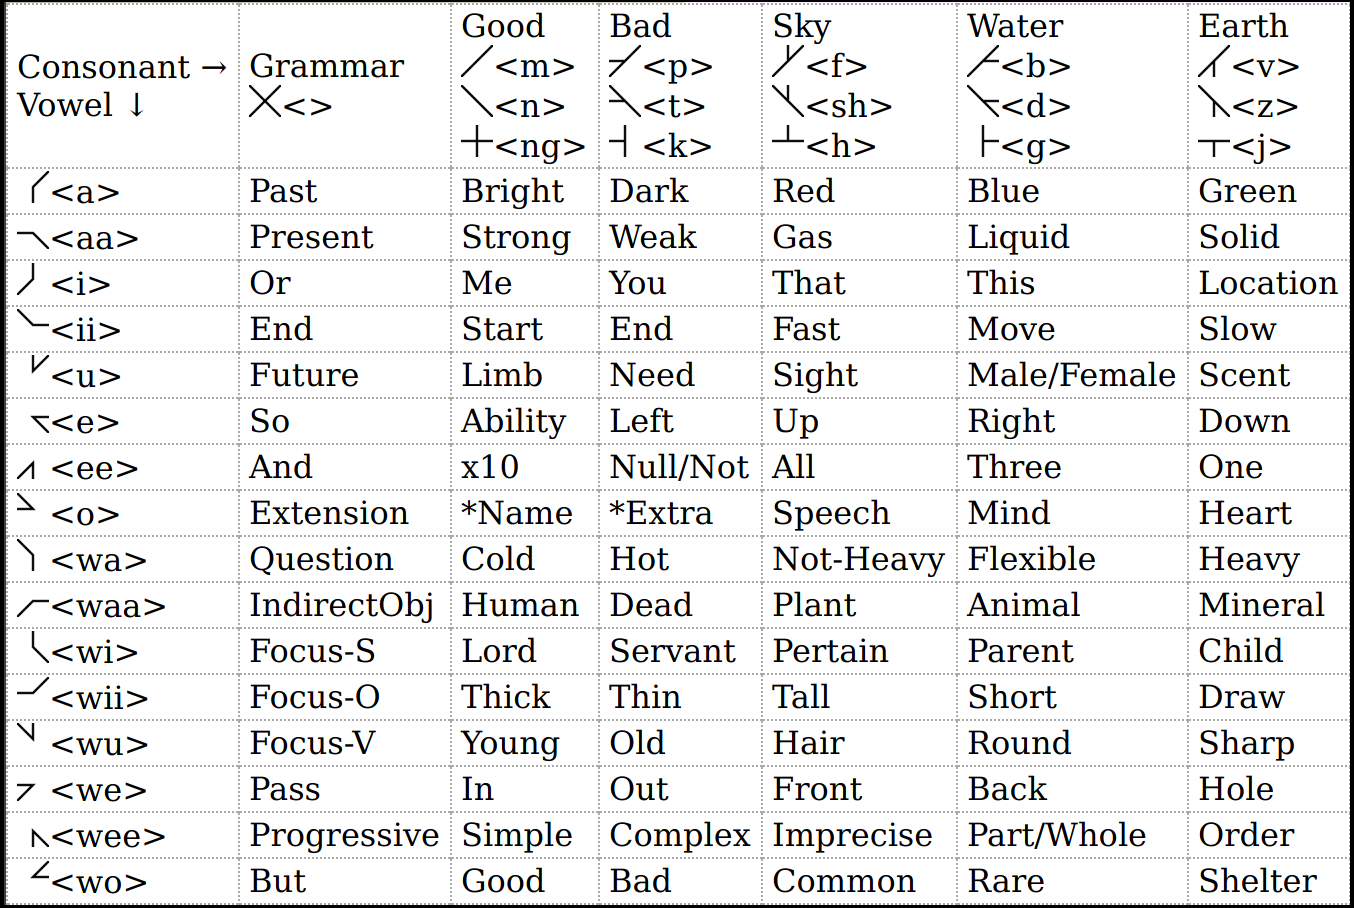
\includegraphics[width=4.0in]{language.png}
\end{figure}
\clearpage

\chapter{Origin of Fobwa Manuscripts}
In 1896, Pacoitz' worked in a restaurant located in South Dakota. But he tired of cooking and quit his job to take a vacation. (This is what Pacoitz claims, but I think it more likely that he was fired.) After a week, he found a cave in South Dakota wherein he discovered some Fobwa writing on the cave wall. Exploring further, he found some clay jars which had some poems and some historical documents as well as the original text to \emph{the Fall of King Mwefu} in them. And after working on it for a couple years he had deciphered the language.

Many found it odd that Pacoitz had discovered a language that no linguist had ever seen before and that he was able to translate it without any formal training. Now, some people have theorized that Fobwa's emergence as a language, and the fact that only Pacoitz has found any major texts in that language, proves that he fabricated the language, the narratives and other documents. I shouldn't need to tell you how ridiculous this is, but since you're reading this edition instead of another, perhaps you might need me to explain. Pacoitz is constantly mistranslating phrases from the original text as well as changing various aspects about the story; if he really had written both, then he would know how to read it and would not cut out important sections from it. If Pacoitz had written the original text, then one would expect the original to be shorter both because it's a lot more work to write in Fobwa and because Pacoitz only seem to care about his English translation.

Pacoitz is just not creative enough to come up with anything original, let alone create an elaborate well-thought-out hoax to purport a translation of what would be fake documents written in a fake language.

Not a single scholar of any standing finds any of \emph{the Elevated Pacoitz Doctrine} (As some call it) to have even an inkling of credibility. The texts have all the evidence of older productions; Joshua Greenberg confirmed the works (via carbon dating some excess paper) to be at least 1,300 years old. So it is highly probable that Fobwa, and \emph{The Fall of King Mwefu} are historical works and not apocryphal.



\end{document}
